%!TEX root = ../../main.tex

\chapter{Model Checking}
\label{chap_mc}

\targets{
  \item Understand the basic principles of Model Checking
  \item Know how to apply Model Checking for Software Verification
  \item Get to know a state-of-the art Software Model Checking tool CPAchecker
}

\newcommand\hl[1]{
  \relax
  \ifmmode
  \bm{#1}
  \else
  {\bfseries #1}
  \fi
}

\newcommand\m[1]{{$#1$}}
\def\sema#1{\lbrack\!\lbrack{#1}\rbrack\!\rbrack}

\newcommand{\tc}[2]{\textcolor{#1}{#2}}

\def\mag#1{\tc{magenta}{#1}}
\def\blue#1{\tc{blue}{#1}}
\def\red#1{\tc{red}{#1}}

\newcommand{\gray}[1]{{\color{lightgray}#1}}

\def\tuple#1{\langle#1\rangle}

\def\F{\mathop{\bf F}\nolimits}
\def\G{\mathop{\bf G}\nolimits}
\def\W{\mathbin{\bf W}}
\def\R{\mathbin{\bf R}}


\definecolor{oceangreen}{RGB}{0,75,90}

\tikzstyle{highlight}=[fill=oceangreen!30]
\tikzstyle{alert}=[fill=red!50]
\tikzstyle{bad}=[fill=red!50]

\tikzstyle{block} = [rectangle, draw, fill=blue!20, ultra thin, 
    text centered, rounded corners, minimum width=4cm, minimum
    height=0.8cm] 

\tikzstyle{ellblock} = [ellipse, draw, fill=green!20, ultra thin, text
centered]
    
\tikzstyle{line} = [draw, -latex']

\tikzset{onslide/.code args={<#1>#2}{%
  \only<#1>{\pgfkeysalso{#2}} % \pgfkeysalso doesn't change the path
}}

\tikzset{hide on/.code={
  \only<#1>{\color{white}}
}}


\tikzset{loc/.style={%
      state,
      minimum width=0.65cm,
      minimum height=0.65cm,
      label distance=-1mm      
    }
}

\tikzset{artloc2/.style 2 args={state, minimum width=0.65cm, minimum
height=0.65cm, label distance=-1mm, align=center,
label=0:{\color{blue}\scriptsize{#1#2}} } }

\tikzset{artloc/.style 2 args={state, minimum width=0.65cm, minimum
height=0.65cm, align=center, label=70:{\color{blue}\scriptsize{#1#2}}
    } }

\tikzset{trans/.style={%
    ->,
    draw,
      font=\scriptsize,           
    }
}


\tikzset{tlbl/.style={%   
      align=left           
    }
}

% Predicates set on slide
\tikzset{pons/.code args={<#1>#2}{%
  \only<#1>{\pgfkeysalso{artloc={$\{ #2 \}$}}} % \pgfkeysalso doesn't change the
  % path
}}

% Model Checking
%!TEX root = ../../../main.tex

\section{Introduction}

\begin{frame}{What does ``Model-Checking'' mean?}
\only<1> {
  \centerline{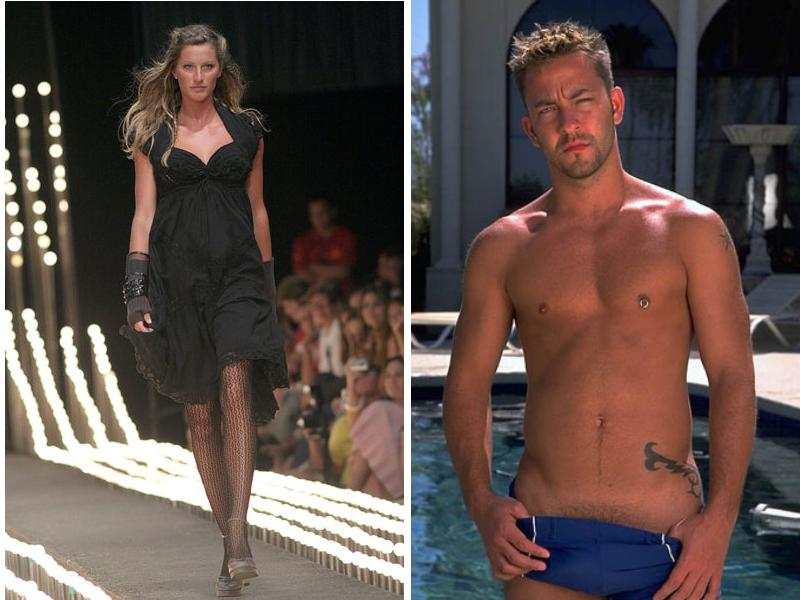
\includegraphics[width=.8\textwidth]{content/chapter_model_checking/model_checking/images/models}}
}

\only<2> {
  \centerline{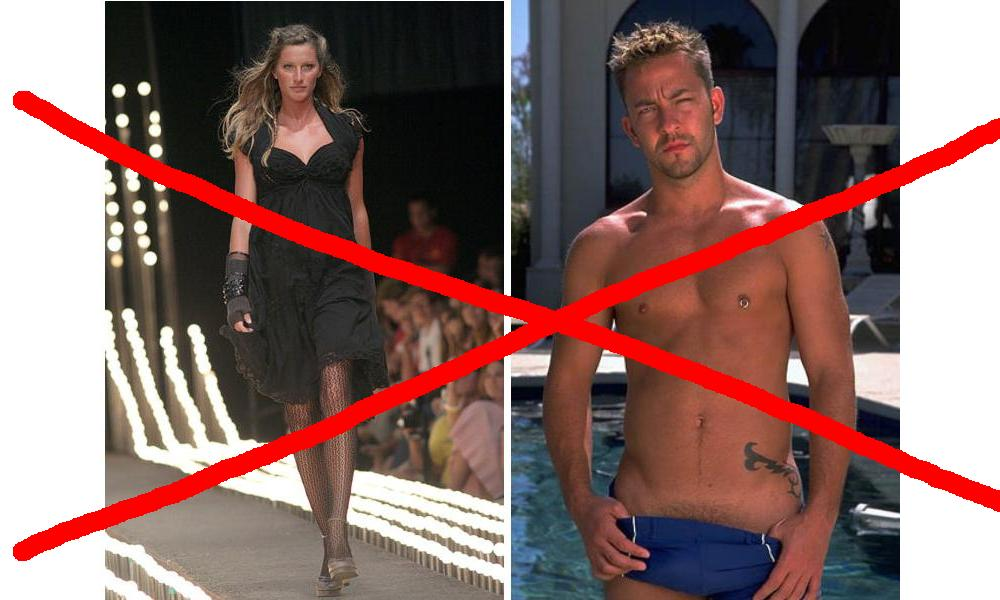
\includegraphics[width=\textwidth]{content/chapter_model_checking/model_checking/images/models1}}
}

\only<3-> {
  \begin{itemize}
    \item \hl{A technical term from logic}
    \item Temporal logic: extension of predicate logic
    \item In german: ``Modellpr"ufung'' (rarely used)
  \end{itemize}
}
\end{frame}

% ----------------------------------------------------------------------

\begin{frame}{Propositional logic (Syntax)}
Formulae of propositional logic consist of \hl{atomic propositions}, e.g.
\bigskip
\begin{itemize}
  \itemsep1em
  \item[] $\mathbf{A}$ \quad $\widehat=$ \quad ``Anna is an architect''
  \item[] $\mathbf{B}$ \quad $\widehat=$ \quad ``Bruno is a bear''
\end{itemize}
\bigskip
and \hl{connectives}, e.g.\ $\land$ (``and''),
    $\lor$ (``or''), $\neg$ (``not''),
    $\to$ (``implies'').
\end{frame}

% ----------------------------------------------------------------------

\begin{frame}{Semantics of propositional logic}

A \hl{valuation} $\mathcal{B}$ is a function assigning 
a \hl{truth value} (\hl{1} or \hl{0}) to each atomic proposition.

\bigskip
The \hl{semantics} of a formula (defined inductively) is the set of valuations
making the formula ``true'' and denoted $\sema{F}$.

\begin{itemize}
  \item[] if \m{F=A} then \m{\sema{F}=\{\,\mathcal{B}\mid\mathcal{B}(A)=1\,\}};
  \item[] if \m{F=F_1 \land F_2} then \m{\sema{F}=\sema{F_1}\cap\sema{F_2}}; \ldots
\end{itemize}

\bigskip
Other notations: $\mathcal{B}\models F$ iff $\mathcal{B}\in\sema{F}$.\\
We say: ``\m{\mathcal{B}} fulfils \m{F}'' or ``\m{\mathcal{B}} is a model of \m{F}''.
\end{frame}

% ----------------------------------------------------------------------

\begin{frame}{The model-checking problem in propositional logic}
\hl{Problem:} Given a valuation \m{\mathcal{B}}
   and a formula \m{F} of propositional logic;

\begin{center}
check whether \m{\mathcal{B}} is a model of \m{F}.
\end{center}   


\hl{Solution}:
\begin{quote}
Replace the atomic propositions by their truth values in \m{\mathcal{B}},
then use a truth table to evaluate to \m{1} or \m{0}.
\end{quote}

\bigskip
\hl{Examples:} 
\begin{itemize}
  \item Let \m{\mathcal{B}_1(A)=1} and \m{\mathcal{B}_1(B)=0}.
  Then \m{\mathcal{B}_1\not\models A\land B} and \m{\mathcal{B}_1\models\neg B}

  \item Let \m{\mathcal{B}_2(A)=1} and \m{\mathcal{B}_2(B)=1}. 
  Then \m{\mathcal{B}_2\models A\land B} and \m{\mathcal{B}_2\not\models\neg B}.
\end{itemize}

\end{frame}

% ----------------------------------------------------------------------

\begin{frame}{Temporal logic}

Takes into account that truth values of atomic proposition may
change with time (the ``world'' transforms).

\bigskip
Example: Truth values of \m{A} in the course of Anna's life:

\begin{center}
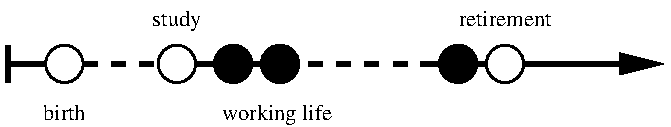
\includegraphics[width=\textwidth]{content/chapter_model_checking/model_checking/images/anna}
\end{center}

Possible statements:
\begin{itemize}
\item Anna will \hl{eventually} be an architect (at some point in the future).
\item Anna is an architect \hl{until} she retires.
\end{itemize}
$\Longrightarrow$ Extension of propositional logic with
    temporal connectives (eventually, until)
\end{frame}

% ----------------------------------------------------------------------

\begin{frame}{Preview}
\hl{Linear-time temporal logics} (example: LTL)
\begin{itemize}
\item formulae with temporal operators
\item evaluated w.r.t.\ (infinite) sequences of valuations
\item Model-checking problem for LTL: Given an LTL formula and a
   sequence of valuations, check whether the sequence is a model
   of the formula.
\end{itemize}

\bigskip
\hl{Computation-tree logic} (CTL, CTL${}^*$)
\begin{itemize}
\item Considers (infinite) \emph{trees} of valuations.
\item Interpretation: non-determinism; multiple possible developments.
\end{itemize}

\end{frame}

% ----------------------------------------------------------------------

\begin{frame}{Connection with program verification}

\hl{State space} of a program:
\begin{itemize}
\item value of program counter
\item contents of variables
\item contents of stack, heap, \ldots
\end{itemize}

\bigskip
Possible atomic propositions:
\begin{itemize}
\item ``Variable $x$ has a positive value.''
\item ``The program counter is at label~$\ell$.''
\end{itemize}

\bigskip
Given a set of atomic propositions, each program state gives rise to a valuation!

\end{frame}

% ---------------------------------------------------------------------- 

\begin{frame}{Programs and temporal logics}

\hl{Linear-time temporal logic}:
\begin{itemize}
\item Each program execution yields a \hl{sequence} of valuations.
\item Interpretation of the program: the set of possible sequences
\item Question of interest: Do all sequences satisfy a given LTL formula?
\end{itemize}

\bigskip
\hl{Computation-tree logic}:
\begin{itemize}
\item The program may branch at certain points, its possible executions
   yield a \hl{tree} of valuations.
\item Interpretation of the program: tree with the (valuation of the)
   initial state as its root
\item Question of interest: Does this tree satisfy a given CTL formula?
\end{itemize}

\bigskip
Thus:
\begin{center}
\hl{verification problem} \ \ $\widehat=$ \ \ \hl{model-checking problem}
\end{center}

\end{frame}


% ----------------------------------------------------------------------

\begin{frame}{Model checking}

Apart from its definition in terms of logic, the term \hl{model checking} is generally understood to mean methods that
\begin{itemize}
\item \hl{verify} whether a given system satisfies a given specification;
\item work \hl{automatically};
\item either prove \hl{correctness} of the system w.r.t.\ to the specification;
\item or exhibit a \hl{counterexample}, i.e.\ an execution violating the
   specification (at least in the linear-time framework).
\end{itemize}

\end{frame}

% ----------------------------------------------------------------------

\begin{frame}{Pros and cons of model checking}

\hl{Advantages:}
\begin{itemize}
\item works automatically(!)
\item suitable for reactive, concurrent, distributed systems
\item can check temporal-logic properties, not just reachability
\end{itemize}

\bigskip
\hl{Disadvantages:}
\begin{itemize}
  \item programs are Turing powerful $\rightarrow$ \hl{undecidability}
    Solution: consider decidable sub-classes
  
  \item state space is huge $\rightarrow$ \hl{computationally expensive}
    Solution: efficient data structures and algorithms
\end{itemize}
\end{frame}

% ----------------------------------------------------------------------

\begin{frame}{Problems with model checking}

  \begin{itemize}
    \item For the aforementioned problems we cannot hope to verify arbitrary
   properties of arbitrary programs!

    \item Possibly we must consider a simplified mathematical model of the system
   of interest that ignores its ``unimportant'' aspects.

    \item Construction of such models and the specification as well as the actual
   verification require \hl{effort} and (possibly high) \hl{cost}.

    \item $\Rightarrow$ useful in early design phases

    \item $\Rightarrow$ economic gain for critical systems where failure is
   costly (CPUs, communication protocols, aircraft, \ldots)
  \end{itemize}
\end{frame}



%!TEX root = ../../../main.tex

\section{Kripke structures}

% ---------------------------------------------------------------------

\begin{frame}{System model}

We shall use a very generic (and unspecific) model, i.e.
  \hl{transition systems}, essentially directed graphs:

\begin{equation*}
  {\cal T}=(S,\mathord{\to},r)
\end{equation*}
  
\bigskip
 $\mathbf{S}\qquad\qquad\qquad\>\>\>\widehat=\qquad$
  \hl{state space}; 
  \\ \vspace{.1cm}\quad\quad {\small states that the system may attain (finite or infinite set)}

  \bigskip
 $\mathbf{\mathord{\to}\subseteq S\times S}\qquad\>\widehat=\qquad$
   \hl{transition relation}; 
   \\ \vspace{.1cm}\quad\quad {\small describes which actions or ``steps'' are possible}
  
  \bigskip
 $\mathbf{r\in S}\qquad\qquad\,\ \ \ \widehat=\qquad$
    \hl{initial state} (``root'')

\end{frame}


% ---------------------------------------------------------------------

\begin{frame}{Example 1: Producer/Consumer}

(Pseudocode) program with variables and concurrency:

\bigskip
$\mbox{{\bf var} \  {\it turn} \  \{0,1\} \  {\bf init} \  0;}$\\
$\mbox{{\bf cobegin} } \:\{ \tc{blue}{P} \parallel \tc{magenta}{K} \} \: \mbox{ {\bf coend}}$


\bigskip
$\tc{blue}{P} = $ \tc{blue}{%\hspace{.1cm}
\begin{minipage}[t]{4cm}
\begin{tabbing}
colu \= co \= colu \= \kill
{\bf start}; \\
{\bf while} {\bf true} {\bf do} \\
\> $w_0$: \> {\bf wait} $({\it turn} = 0)$; \\
\> $p_0$: \> /* produce */ \\
\>        \> ${\it turn} := 1$; \\
{\bf od};\\
{\bf end}
\end{tabbing}
\end{minipage}}
%\hspace{.5cm}
$\tc{magenta}{K} = $ \tc{magenta}{%\hspace{.01cm}
\begin{minipage}[t]{4cm}
\begin{tabbing}
colu \= co \= colu \= \kill
{\bf start}; \\
{\bf while} {\bf true} {\bf do} \\
\> $w_1$: \> {\bf wait} $({\it turn} = 1)$; \\
\> $c_1$: \> /* consume */ \\
\>        \> ${\it turn} := 0$; \\
{\bf od};\\
{\bf end}
\end{tabbing}
\end{minipage}}
\end{frame}


% ---------------------------------------------------------------------

\begin{frame}{Example 1: Corresponding transition system}

$S = \tc{blue}{\{w_0,p_0\}}\times\tc{magenta}{\{w_1,c_1\}}\times\{0,1\}$;
  \quad Initial state: $(w_0,w_1,0)$

\bigskip
\begin{center}
  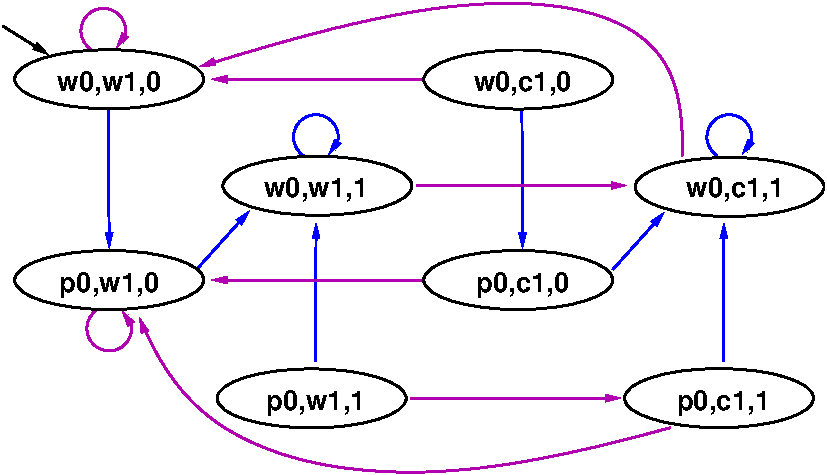
\includegraphics[width=\textwidth]{content/chapter_model_checking/model_checking/images/mutex-ts}
\end{center}

\end{frame}


% ---------------------------------------------------------------------
\begin{frame}{Example 2: Petri net}

State space = set of markings\\[1cm]

\setlength{\unitlength}{.025\textwidth}\hfil%
\begin{picture}(18,12.5)(0,0)
%place and transition symbols
\multiput(1,3)(8,0){3}{\circle2}\multiput(4,2)(8,0){2}{\framebox(2,2){}}
\multiput(1,9.5)(8,0){2}{\circle2}\put(4,8.5){\framebox(2,2){}}
% place labels
\put(0,0){\makebox(2,1.5)[t]{\blue{$p_1$}}}
\put(8,0){\makebox(2,1.5)[t]{\blue{$p_3$}}}
\put(16,0){\makebox(2,1.5)[t]{\blue{$p_5$}}}
\put(0,11){\makebox(2,1.5)[b]{\blue{$p_2$}}}
\put(8,11){\makebox(2,1.5)[b]{\blue{$p_4$}}}
% transition labels
\put(4,0){\makebox(2,1.5)[t]{\blue{\small$t_1$}}}
\put(12,0){\makebox(2,1.5)[t]{\blue{\small$t_3$}}}
\put(4,11){\makebox(2,1.5)[b]{\blue{\small$t_2$}}}
% initial marking
\multiput(1,3)(0,6.5){2}{\circle*{.5}}
% arcs
\multiput(2,3)(4,0){4}{\vector(1,0){2}}
\multiput(2,9.5)(4,0){2}{\vector(1,0){2}}
\put(7,8.5){\oval(12,4.5)[lb]}\put(7,4){\oval(12,4.5)[rt]}
\put(13,4){\vector(0,-1){0}}
\end{picture}\hfil%
\setlength{\unitlength}{.025\textwidth}\hfil%
\begin{picture}(16,12.5)(0,0)
% transitions
\multiput(6,1.5)(-4,5.5){2}{\vector(1,1){4}}
\multiput(8,1.5)(-4,5.5){2}{\makebox(2,2)[lt]{\blue{\small$t_1$}}}
\multiput(6,1.5)(4,5.5){2}{\vector(-1,1){4}}
\multiput(2,1.5)(4,5.5){2}{\makebox(2,2)[rt]{\blue{\small$t_2$}}}
\put(10,7){\vector(1,1){4}}\put(12,7){\makebox(2,2)[lt]{\blue{\small$t_3$}}}
% markings
\put(4,0){\makebox(4,1.5){$\to$\ \blue{$\tuple{1\!,1\!,0\!,0\!,0}$}}}
\put(0,5.5){\makebox(4,1.5){\blue{$\tuple{1\!,0\!,0\!,1\!,0}$}}}
\put(8,5.5){\makebox(4,1.5){\blue{$\tuple{0\!,1\!,1\!,0\!,0}$}}}
\put(4,11){\makebox(4,1.5){\blue{$\tuple{0\!,0\!,1\!,1\!,0}$}}}
\put(12,11){\makebox(4,1.5){\blue{$\tuple{0\!,0\!,0\!,0\!,1}$}}}
\end{picture}\hfil
\end{frame}

% ---------------------------------------------------------------------

\begin{frame}{Implicitly given transition systems}
\begin{itemize}
\itemsep1em
\item Quite often, a transition system is given to us ``implicitly'',
   i.e.\ in the form of a program, from which we extract the
   transition system.

\item In such a setting, we are given an initial state and a function
   for computing the direct successor states of a given state, such that
   transitions are computed only on demand.

\item Some of our analysis methods will be suitable for such a setting.
\end{itemize}
\end{frame}

% ----------------------------------------------------------------------

\begin{frame}{Finite and infinite transition systems}

In principle, a transition system many have infinitely many states.
Some of the possible reasons are:
\bigskip

\begin{itemize}
\item \hl{Data:} integers, reals, lists, trees, pointer structures, \ldots
\item \hl{Control:} (recursive) procedures, dynamic thread creation, \ldots
\item \hl{Communication:} unbounded FIFO channels, \ldots
\item \hl{Unknown parameters}: number of participants in a protocol, \ldots
\item \hl{Real time}: discrete or continuous time
\end{itemize}

\bigskip
 Some (not all!) of these features lead to \red{Turing-powerful}
 computation models (and thus \red{undecidable}
 verification problems).

\end{frame}

% ----------------------------------------------------------------------

\begin{frame}{Example: Petri net}
Petri nets may have an infinite state space, too:

\bigskip
\begin{center}
{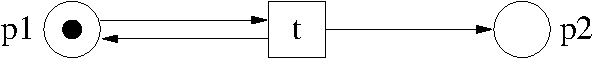
\includegraphics[width=\textwidth]{content/chapter_model_checking/model_checking/images/infinite}}
\end{center}

\bigskip
Reachable states are:
\blue{$\tuple{1,0},\ \tuple{1,1},\ \tuple{1,2},\ \ldots$}

\bigskip
Reachability and LTL decidable, CTL undecidable.

\end{frame}

% ---------------------------------------------------------------------

\begin{frame}{Finite Kripke structures}
\begin{itemize}
\itemsep1em
\item For now, we restrict ourselves to finite state spaces.

\item Finite systems: e.g.\ hardware systems, programs with finite
   data typs (Boolean programs), certain communication protocols, \ldots

\item Finite systems may also be obtained by \hl{abstracting} an
   infinite system.

\item Remaining problem: \red{state-space explosion},
   systems may be finite but VERY large.   
\end{itemize}
\end{frame}

% ---------------------------------------------------------------------

\begin{frame}{Reasons for state-space explosion (1)}

A common reason is \hl{concurrency}.

\bigskip
\hl{Example}: Consider the following Petri net:

\bigskip
\begin{center}
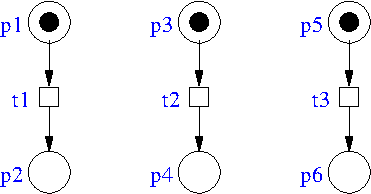
\includegraphics[width=.8\textwidth]{content/chapter_model_checking/model_checking/images/3prozesse}
\end{center}

\end{frame}

% ---------------------------------------------------------------------

\begin{frame}{}

The reachability graph has got \blue{$8=2^3$} states and \blue{$6=3!$}
paths.

\bigskip
\begin{center}
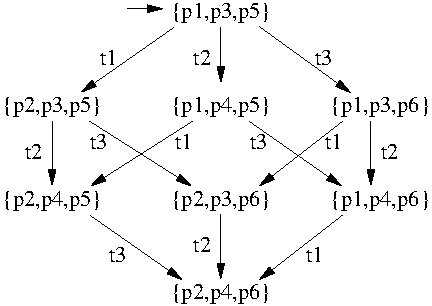
\includegraphics[width=.8\textwidth]{content/chapter_model_checking/model_checking/images/3pkrip}
\end{center}

\bigskip
With \blue{$n$} components we have \blue{$2^n$} states and \blue{$n!$} paths.

\end{frame}

% ---------------------------------------------------------------------

\begin{frame}{Reasons for state-space explosion (2)}

A second common reason is \hl{data}.
\begin{itemize}
  \item e.g.\ programs with few large or many small variables
  \item size of state space: 2 to the number of bits
\end{itemize}

\bigskip
Counteractions:
\begin{itemize}
\item \hl{Abstraction}: ignore ``unimportant'' data
\item \hl{Compression}: work with \emph{sets} of states;
  efficient data structures for storing and manipulating sets
\item \hl{Approximation}: find over- or underapproximations of the
  reachable states
\end{itemize}

\end{frame}

% ---------------------------------------------------------------------

\begin{frame}{Kripke structures}

Idea: Extract from each state a \hl{valuation}.
\begin{center}
$${\cal K} = (S,\mathord{\to},r,AP,\nu)$$
\end{center}

\begin{align*}
(S,\mathord{\to},r) \quad \widehat= \quad  &
   \text{underlying \hl{transition system}} \\
AP \quad  \widehat= \quad &
   \text{set of \hl{atomic propositions}} \\
\nu\colon S \to 2^{AP} \quad  \widehat= \quad &
   \text{\hl{interpretation} of atomic propositions} \\
& \text{(``valuation'')}
\end{align*}

\bigskip 
Remarks:
\begin{itemize}
\item $2^{AP}$ denotes the \emph{powerset} of $AP$.
\item Valuations are represented here as subsets of \m{AP} rather
   than functions; the propositions contained in the set are
   those that are deemed true.
\end{itemize}
\end{frame}

% ---------------------------------------------------------------------

\begin{frame}{Example of a Kripke structure}
\begin{itemize}
\itemsep1em
\item Transition system $(S,\mathord{\to},r)$ as in Example~1.

\item Suppose we are interested in the acts of production and consumption.

\item Sei $AP = \{\tc{blue}{{\it prod}},\tc{magenta}{{\it cons}}\}$;

\item $\nu^{-1}(\blue{\it prod}) = \tc{blue}{\{p_0\}}\times\tc{magenta}{\{w_1,c_1\}}\times\{0,1\}$;

\item $\nu^{-1}(\mag{\it cons}) = \tc{blue}{\{w_0,p_0\}}\times\tc{magenta}{\{c_1\}} \times\{0,1\}$.
\end{itemize}  
\end{frame}

% ---------------------------------------------------------------------

\begin{frame}{}
The valuations in Example~1:

\bigskip
\begin{center}
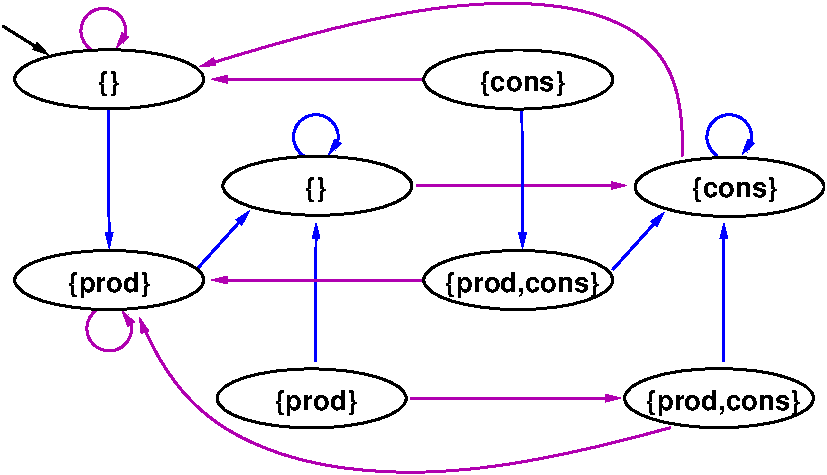
\includegraphics[width=\textwidth]{content/chapter_model_checking/model_checking/images/mutex-krip}
\end{center}

\end{frame}

% ---------------------------------------------------------------------

\begin{frame}{Sequences and trees of valuations}
In \hl{linear-time logic} we consider the possible valuation sequences:

\begin{quote}
z.B.\ \quad \blue{$\emptyset\ \emptyset\ \{{\it prod}\}\ \emptyset\ \{{\it cons}\} \ldots$}
\quad oder \quad
\blue{$\emptyset\ \{{\it prod}\}\ \{{\it prod}\}\ \{{\it prod}\}\ \ldots$}
\end{quote}

\bigskip
In \hl{computation-tree logic} we consider the ``tree-wise unfolding''
   of the Kripke structure:
\begin{center}
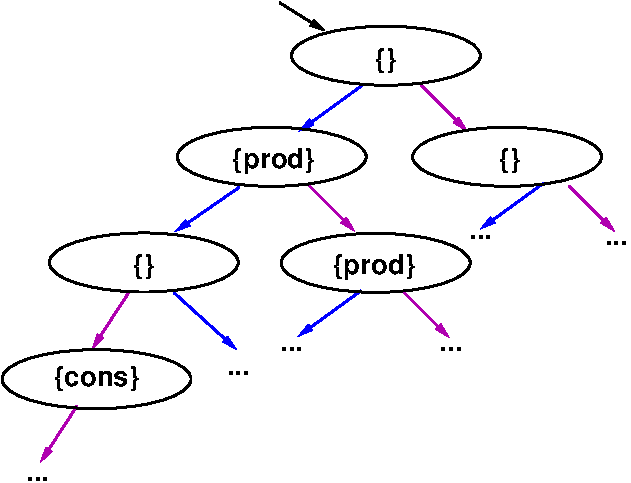
\includegraphics[height=4cm]{content/chapter_model_checking/model_checking/images/mutex-tree}
\end{center}   
\end{frame}

% ---------------------------------------------------------------------

\begin{frame}{Examples of temporal-logic properties}

\hl{``It is never possible that \blue{\it prod}
  and \mag{\it cons} hold at the same time.''}
\begin{quote}
Intuitively, this property holds because no state in which
both \blue{\it prod} and \mag{\it cons} holds is reachable
from the beginning, which can be verified by inspecting the
sequences and trees.
\end{quote}
A property of this form is also called an \hl{invariant}.

\bigskip
\hl{``Whenever something is produced it may be consumed afterwards.''}
\begin{quote}
We may take the view that this property does not hold because of
the following sequence:
\blue{$\emptyset\ \{{\it prod}\}\ \emptyset\ \emptyset\ \emptyset \ldots$}
Thus, something is produced but followed by an infinite loop.
\end{quote}
A property of this form is also called a \hl{reactivity property}.
\end{frame}

% ---------------------------------------------------------------------

\begin{frame}{Fairness}
\begin{itemize}
\item We may also take the view that the second property merely fails
   because of overly simplistic modelling:
\item In the counterexample, only one process is acting, making ``empty''
   steps, while the second process does not do anything.
\item Such a behaviour is usually unrealistic in concurrent systems;
   even if one process may be faster than another and execute multiple
   steps, a ``fair'' scheduler will eventually grant execution time
   to either process.
\item We may therefore wish to exclude such unrealistic (``unfair'') executions
   and only consider ``fair'' ones. In other words, we work under certain
   ``fairness assumptions''.
\item Under a reasonable fairness assumption, the second property holds.
\end{itemize}
\end{frame}

% ---------------------------------------------------------------------


%!TEX root = ../../../main.tex

\section{Linear-time logic}

% ---------------------------------------------------------------------

\begin{frame}{Preliminaries}

\hl{Linear-time logic} in general:
\begin{itemize}
\item any logic working with sequences of valuations
\item model: time progresses in discrete steps and in linear fashion, each point in time has exactly one possible future
\item origins in philosophy/logic
\end{itemize}

\bigskip
Most prominent species: \hl{LTL}
\begin{itemize}
\item in use for verification since end of the 1970s
\item \hl{spezification} of correctness properties
\end{itemize}
\end{frame}

% ---------------------------------------------------------------------

\begin{frame}{Recap}
\begin{itemize}
\itemsep1em
\item Let \m{AP} be a set of atomic propositions.

\item \m{2^{AP}} denotes the powerset of \m{AP},
   i.e.\ its set of subsets.

\item \m{(2^{AP})^\omega} denotes the set of
  (infinite) sequences of valuations (of \m{AP}).\\[20mm]
\end{itemize}
\end{frame}

% ---------------------------------------------------------------------

\begin{frame}{Syntax of LTL}

Let $AP$ be a set of atomic propositions. The set of \hl{LTL formulae} over $AP$ is inductively defined as follows:

\bigskip
\begin{itemize}
\itemsep1em
\item If $p\in AP$ then $p$ is a formula.

\item If $\phi_1,\phi_2$ are formulae then so are:
\item[] $\neg\phi_1, \qquad \phi_1\lor\phi_2, 
\qquad \hl{\X}\phi_1, \qquad \phi_1\hl{\U}\phi_2$
\end{itemize}

\bigskip
Intuitive meaning:
$\hl{\X}\>\widehat{=}\>$ ``next'',
$\hl{\U}\>\widehat{=}\>$ ``until''.

\end{frame}

% ---------------------------------------------------------------------

\begin{frame}{Semantics of LTL}

Let \m{\phi} be an LTL formula and \m{\sigma} a valuation sequence.\\
We write \m{\sigma\models\phi} for ``\m{\sigma} satisfies \m{\phi}.''

 \begin{center}
  \(\begin{array}[t]{rl@{\hskip2em}l}
    \sigma\models & p & \hbox{if \m{p\in AP} and $p\in \sigma(0)$} \\
    \sigma\models & \neg\phi & \hbox{if $\sigma\not\models\phi$}\\
    \sigma\models & \phi_1\lor\phi_2 & \hbox{if
  $\sigma\models\phi_1$ or $\sigma\models\phi_2$}\\
    \sigma\models & \hl{\X}\phi & \hbox{if $\sigma^1\models\phi$}\\
    \sigma\models & \phi_1\hl{\U}\phi_2 & \hbox{if \m{\exists i\colon
    \big(\sigma^i\models\phi_2
   \ \ \land \ \ \forall k<i\colon \sigma^k\models\phi_1\big)}}\\
    \end{array}\)
\end{center}

\bigskip
Semantics of \m{\phi}: \qquad
  $\sem{\phi} = \{\,\sigma\mid\sigma\models\phi\,\}$

\end{frame}

% ---------------------------------------------------------------------

\begin{frame}{Examples}

Let \m{AP=\{p,q,r\}}. Find out whether the sequence
    $$\sigma=\{p\}\ \{q\}\ \{p\}^\omega$$
 satisfies the following formulae:

\begin{center}\(\begin{array}[t]{c}
p \\
q \\
\hl{\X} q \\
\hl{\X} \neg p  \\
p \hl{\U} q  \\
q \hl{\U} p  \\
(p\lor q) \hl{\U} r 
\end{array}\)\end{center}

\end{frame}

% ---------------------------------------------------------------------

\begin{frame}{Extended syntax}
We commonly use the following abbreviations:

\bigskip\small
  \(\begin{array}[t]{rcl@{\quad}rcl}
      \phi_1\land\phi_2 & \equiv & \neg(\neg\phi_1\lor\neg\phi_2) &
      \F\phi            & \equiv & {\bf true}\U\phi\\
      \phi_1\to\phi_2   & \equiv & \neg\phi_1\lor\phi_2 &
      \G\phi            & \equiv & \neg\F\neg\phi\\
      {\bf true}        & \equiv & a\lor\neg a &
      \phi_1\W\phi_2    & \equiv & (\phi_1\U\phi_2)\lor\G\phi_1\\
      {\bf false}       & \equiv & \neg{\bf true} &
      \phi_1\R\phi_2    & \equiv & \neg(\neg\phi_1\U\neg\phi_2)\\
    \end{array}\)

\bigskip
Meaning:
$\F\>\widehat{=}\>$ ``finally'' (eventually),\ \ 
$\G\>\widehat{=}\>$ ``globally'' (always),\\
\ \phantom{Meaning:}%
$\W\>\widehat{=}\>$ ``weak until'',\ \ 
$\R\>\widehat{=}\>$ ``release''.

\end{frame}

% ---------------------------------------------------------------------

\begin{frame}{Some example formulae}

\hl{Invariant:} $\G \neg(\mathit{cs}_1 \wedge \mathit{cs}_2)$
\begin{itemize}
  \item $cs_1$ and $cs_2$ are never true at the same time.
\end{itemize}
Remark: This particular form of invariant is also called
  \hl{mutex property} (``mutual exclusion'').

\bigskip
\hl{Safety:} $(\neg x)\W y$
\begin{itemize}
\item $x$ does not occur before y has happend.
\end{itemize}
Remark: It may happen that $y$ never happens in which case $x$
  also never happens.

\bigskip
\hl{Liveness:} $(\neg x)\hl{\U} y$
\begin{itemize}
\item $x$ does not occur before $y$
   \red{and} $y$ eventually happens.
\end{itemize}

\end{frame}

% ---------------------------------------------------------------------

\begin{frame}{More examples}

$\G\F p$
\begin{itemize}
\item $p$ occurs infinitely often.
\end{itemize}

$\F\G p$
\begin{itemize}
\item At some point $p$ will continue to hold forever.
\end{itemize}

$\G (\mathit{try_1} \rightarrow \F \mathit{cs_1})$
\begin{itemize}
\item For mutex algorithms: Whenever process~1 tries to enter its
   critical section it will eventually succeed.
\end{itemize}

\end{frame}

% ---------------------------------------------------------------------

\begin{frame}{Tautology, equivalence}
\begin{itemize}
\itemsep1em
\item Certain oncepts from propositional logic
   can be transferred to LTL.

\item \hl{Tautology}: A formula \m{\phi} with \m{\sema{\phi}=(2^{AP})^\omega}
   is called tautology.

\item \hl{Unsatisfiability}: A formula \m{\phi} with \m{\sema{\phi}=\emptyset}
   is called unsatisfiable.

\item \hl{Equivalence}: Two formulae \m{\phi_1,\phi_2} are called equivalent
    iff\ \m{\sema{\phi_1}=\sema{\phi_2}}.\\
    \ \phantom{Equivalence:}Denotation: \m{\phi_1\equiv\phi_2}
\end{itemize}
\end{frame}

% ---------------------------------------------------------------------

\begin{frame}{Equivalences: relations between operators}
$$\begin{array}{rcl}
\hl{\X} (\phi_1 \vee \phi_2) & \equiv & \hl{\X} \phi_1 \: \vee \: \hl{\X} \phi_2   \\
\hl{\X} (\phi_1 \wedge \phi_2) & \equiv & \hl{\X} \phi_1 \: \wedge \: \hl{\X} \phi_2   \\
\hl{\X} \neg \phi & \equiv & \neg \hl{\X} \phi \\[0.3cm]
\F (\phi_1 \vee \phi_2) & \equiv & \F \phi_1 \: \vee \: \F \phi_2   \\
\neg \F \phi& \equiv & \G \neg \phi \\[0.3cm]
\G (\phi_1 \wedge \phi_2)&\equiv & \G \phi_1 \: \wedge \: \G \phi_2 \\
\neg \G \phi& \equiv & \F \neg \phi \\[0.3cm]
(\phi_1 \wedge \phi_2) \hl{\U} \psi & \equiv & (\phi_1 \hl{\U} \psi) \: \wedge \: (\phi_2 \hl{\U} \psi)\\
\phi \hl{\U} (\psi_1 \vee \psi_2) & \equiv & (\phi \hl{\U} \psi_1) \: \vee \: (\phi \hl{\U} \psi_2)
\end{array}$$
\end{frame}

% ---------------------------------------------------------------------

\begin{frame}{Equivalences: idempotence and recursion laws}
$$\begin{array}{rcl}
\F \phi & \equiv & \F \F \phi    \\[0.3cm]
\G \phi & \equiv & \G \G \phi    \\[0.3cm]
\phi \hl{\U} \psi & \equiv & \phi \hl{\U} (\phi \hl{\U} \psi) \\[2cm]

\F \phi & \equiv & \phi \vee \hl{\X} \F \phi \\[0.3cm]
\G \phi & \equiv & \phi \wedge \hl{\X} \G \phi \\[0.3cm]
\phi \hl{\U} \psi & \equiv & \psi \vee (\phi \wedge \hl{\X} (\phi \hl{\U} \psi)) \\[0.3cm]
\phi \W \psi & \equiv & \psi \vee (\phi \wedge \hl{\X} (\phi \W \psi))
\end{array}$$
\end{frame}

% ---------------------------------------------------------------------

\begin{frame}{Interpretation of LTL on Kripke structures}
\begin{itemize}
\itemsep1em  
\item Let ${\cal K}=(S,\mathord{\to},r,AP,\nu)$ be a Kripke structure.\\
 We are interested in the valuation sequences generated by \m{\cal K}.

\item Let \m{\rho} in \m{S^\omega} be an infinite path of \m{\cal K}.

\item We assign to \m{\rho} an ``image'' $\nu(\rho)$
   in $(2^{AP})^\omega$; for all $i\ge0$ let
  $$\nu(\rho)(i) = \nu(\rho(i))$$
   i.e.\ $\nu(\rho)$ is the corresponding valuation sequence.

\item Let \m{\sema{\cal K}} denote the set of all such sequences:
$$\sema{\cal K} = \{\,\nu(\rho)\mid \hbox{$\rho$ is
    an infinite path of $\cal K$}\,\}$$
\end{itemize}
\end{frame}

% ---------------------------------------------------------------------

\begin{frame}{The LTL model-checking problem}
\begin{itemize}
\itemsep1em
\item\hl{Problem:} Given a Kripke structure
    ${\cal K}=(S,\mathord{\to},r,AP,\nu)$
   and an LTL formula \m{\phi} over \m{AP}, does
  \m{\sema{\cal K}\subseteq\sema{\phi}} hold?

\item\hl{Definition:} If \m{\sema{\cal K}\subseteq\sema{\phi}}
  then we write ${\cal K}\models\phi$.

\item\hl{Interpretation:} \red{Every} execution of \m{\cal K} must 
  satisfy \m{\phi} for \m{{\cal K}\models\phi} to hold.

\item\hl{Remark:} We may have ${\cal K}\not\models\phi$
   \red{and} ${\cal K}\not\models\neg\phi$!
\end{itemize}
\end{frame}

% ---------------------------------------------------------------------

\begin{frame}{Example}

Consider the following Kripke structure \m{{\cal K}} with \m{AP=\{p\}}:

\begin{center}
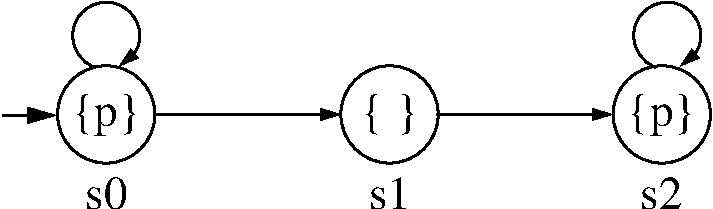
\includegraphics[scale=.4]{content/chapter_model_checking/model_checking/images/ctl-ltl}
\end{center}

\bigskip                  
There are two classes of infinite paths in \m{\cal K}:
\begin{itemize}
\item (i) Either the system stays in \m{s_0} forever,
\item (ii) or it eventually reaches \m{s_2} via \m{s_1} and remains there.
\end{itemize}

\bigskip
We have:
\begin{itemize}
\item \m{{\cal K}\models\F\G p} because all runs eventually end in a state
   satisfying \m{p}.
\item \m{{\cal K}\not\models\G p} because executions of type~(ii) contain
   a non-\m{p} state.
\end{itemize}

\end{frame}

% ---------------------------------------------------------------------

\begin{frame}{Dealing with deadlocks}

The definition of the model-checking problem only considers the
infinite sequences!

\bigskip
Thus, executions reaching a deadlock (i.e.\ a state without any
successor) will be ignored, with possibly unforeseen consequences:
\begin{itemize}
\item Suppose \m{\cal K} contains an error, so that every execution reaches
    a deadlock.
\item Then \m{\sema{\cal K}=\emptyset}, so \m{\cal K} satisfies
   \emph{every} formula, according to the definition.
\end{itemize}

\end{frame}

% ---------------------------------------------------------------------

\begin{frame}{Possible alternatives}

Remove deadlocks by design:
\begin{itemize}
\item equip deadlock states with a self loop
\item Interpretation: system stays in deadlock forever
\item adapt formula accordingly, if necessary
\end{itemize}

\bigskip
Treat deadlocks specially:
\begin{itemize}
\item Check for deadlocks before LTL model checking, deal with them separately.
\end{itemize}

\end{frame}

% ---------------------------------------------------------------------

% Software Model Checking

\newcommand{\vect}[1]
  {\overline #1}

\newcommand{\varset}
  { V }
  
\newcommand{\domain}
  { \mathcal{D} }


% --------------------------------------------------------------
% ---------------------- Logic ---------------------------------
% --------------------------------------------------------------

\newcommand{\satl}
  { \models_{\logic} }

\newcommand{\sat}
  { \models }

\newcommand{\unsat}
  {\not\models}

% --------------------------------------------------------------
% -------------------- Kripke structure ------------------------
% --------------------------------------------------------------

\newcommand{\mstates}{S}
\newcommand{\minits}{I}
\newcommand{\mtrans}{T}  
\newcommand{\mlabels}{\nu}
\newcommand{\mreachables}{R}
\newcommand{\mproperty}{P}

\newcommand{\kripke}{{\cal K}}    
\newcommand{\kripkedef}{\kripke = (\mstates, \mtrans, \minits, AP, \mlabels)}
      
% Type assignment
\newcommand{\ftype}
  { \tau }
  
\newcommand{\type}[1]
  { \ftype(#1) }

% Variable assignment
\newcommand{\fval}
  { v }
\newcommand{\val}[1]
  { v(#1) }
  
% Variable
\newcommand{\var}
  { x \in V}




% --------------------------------------------------------------
% -------------------- State transition system (2) -------------
% --------------------------------------------------------------



\newcommand{\sysdef}
  {S : (V, I, T)}

\newcommand{\sys}
  {S = (I(\vect{x}), T(\vect{x}, \vect{x'})) }

\newcommand{\inv}
  {P(\vect{x})}



% --------------------------------------------------------------
% -------------------- Program  --------------------------------
% --------------------------------------------------------------


\newcommand{\progdef}
  {\langle V,I,T \rangle}
  
\newcommand{\prog}
  {P = \progdef}


% --------------------------------------------------------------
% -------------------- Program (imperative)  -------------------
% --------------------------------------------------------------

% Location
\newcommand{\iprogl}
  {l}
  
% Transition
\newcommand{\iprogt}
  {\tau}
  
% Constraint
\newcommand{\iprogc}
  {\rho}
  
  
  
\newcommand{\iprogsymb}
  {P}

\newcommand{\iprogvars}
  {V}

\newcommand{\iproglocs}
  {L}

  
\newcommand{\iprogtrans}
  {T}

\newcommand{\iprog}
  {\iprogsymb = (\iprogvars, \iproglocs, \iprogl_0, \iprogtrans)}


\newcommand{\iprogstates}
  {S}

\newcommand{\pre}
  {Pre}

\newcommand{\post}
  {Post}


\newcommand{\preop}[1]
  {\pre(#1)}
  
\newcommand{\postop}[1]
  {\post(#1)} 

  
  
  
%-------------- k-Induction definitions ------------------------- 
  
% Simulation relation 
\newcommand{\simul}[1]
  {\preceq_{#1}}

\newcommand{\nsimul}[1]
  {\npreceq_{#1}}
  
\newcommand{\simuld}
  {\simul{d}}
  
\newcommand{\simulr}
  {\simul{r}}


  
% Execution paths

\newcommand{\stateseq}
  {s_0, s_1, \ldots , s_n}

\newcommand{\execpathof}[2]
  {\pi^{#1}(#2)}

\newcommand{\execpath}[1]
  {\execpathof{#1}{s_0, s_1, \ldots, s_n}}

\newcommand{\execpathij}[3]
  {\execpathof{#1}{s_{#2}, \ldots, s_{#3}}}
  
  
% Interpolants

\newcommand{\interp}
  { \mathcal{I} }
  
  
%---------------- Abstraction ------------------------------------

% Abstract elements
\newcommand{\aelems}
  {L} 

% Ordering  
\newcommand{\aorder}
  {\sqsubseteq}

\newcommand{\astrictorder}
  {\sqsubset}



% Definition of the lattice  
\newcommand{\latticedef}
  {\lattsymb = (\aelems, \aorder, \bot, \top, \join, \meet)}


% Abstract domain
\newcommand{\apre}
  {Pre^{\#}}

\newcommand{\apost}
  {Post^{\#}}

\newcommand{\apredef}
  {\apre: \aelems \times T \to \aelems}

\newcommand{\apostdef}
  {\apost: \aelems \times T \to \aelems}

\newcommand{\apreop}[1]
  {\apre(#1)}
  
\newcommand{\apostop}[1]
  {\apost(#1)}

\newcommand{\fconcrete}
  {\sem{\cdot}}

\newcommand{\fconcretedef}
  {\fconcrete: \aelems \to 2^{\mstates}}

\newcommand{\adomain}
  {(\lattice, \fconcrete, \apre, \apost)}





% --------------------------------------------------------------
% -------------------- Slides ----------------------------------
% --------------------------------------------------------------
  
\newcommand{\slidepart}[2]
  {\bigskip \uncover<#1->{#2}}



%!TEX root = ../../../main.tex

\section{Symbolic Model Checking}

% Functional properties of systems

\begin{frame}{Recall}

The functional properties of a software/hardware system can be expressed as
\hl{temporal} properties

\begin{itemize}
  \itemsep1em
  \item for a suitable model of the system, e.g. Kripke structure $\kripkedef$
  \item in a suitable temporal logic, e.g. LTL
\end{itemize}
\end{frame}

% ---------------------------------------------------------------------

\begin{frame}{Main classes of properties}
\begin{itemize}
  \itemsep1em
  \item \hl{Invariance properties}: certain states of the system are
  unreachable
    \begin{itemize}
      \item Reachability analysis
    \end{itemize}
  \item \hl{Safety properties}: certain events never happen
    \begin{itemize}
      \item Generalizes invariants and can be reduced to them
    \end{itemize}  
  \item \hl{Liveness properties}: certain events eventually happens
    \begin{itemize}
      \item Cycle detection (for finite-state systems)
    \end{itemize}
\end{itemize}

\bigskip
We focus on checking invariance properties in Software Model Checking
\end{frame}

% ---------------------------------------------------------------------

\begin{frame}{Invariance properties}

Given a Kripke structure $\kripkedef$

\bigskip
The set $\mreachables$ of \hl{reachable states} of $S$ is the smallest
subset of $\mstates$ satisfying the following constraints:

\bigskip
\begin{enumerate}
  \itemsep1em
  \item $\minits \subseteq \mreachables$ \quad (initial states are reachable)
  \item $\mreachables \bowtie \mtrans \subseteq \mreachables$ \quad
    ($\mtrans$-successors of reachable states are reachable)
\end{enumerate}

\bigskip
A \hl{state property} $\mproperty \subseteq \mstates$ is \hl{invariant} iff
$\mreachables \subseteq \mproperty$


\bigskip
\textbf{Note:} We denote the set $\overline{\mproperty} = \mstates
\setminus \mproperty$ as \hl{``bad states''}
\end{frame}

% ---------------------------------------------------------------------  

\begin{frame}{Checking invariance}
In general, to check that the state property $\mproperty$ is invariant for $\kripke$
it suffices to

\begin{enumerate}
  \itemsep1em
  \item compute $\mreachables$ and
  \item check that $\overline{\mproperty} \bigcap \mreachables = \emptyset$ (no
  bad state is reachable)
\end{enumerate}

\bigskip
\uncover<2->{
This can be done explicitly only if $\kripke$ is finite and relatively small (usually
it is not the case)
}

\bigskip
\uncover<3->{
Alternatively, $\kripke$ can be represented \hl{symbolically} and use
\begin{itemize}
  \item BDD-based methods, \hl{if $\kripke$ is finite}
  \item automata-based methods
  \item logic-based methods
\end{itemize}
}
\end{frame}

% ---------------------------------------------------------------------

\begin{frame}{Logic-based Symbolic Model Checking}
Applicable if the system $\kripke$ can be encoded in some logic (or a fragment
of logic) $\logic$ with decidable entailment $\satl$

\bigskip
\uncover<2->{
($\phi \satl \psi$ iff $\phi \wedge \neg \psi$ is \hl{unsatisfiable} in
$\logic$ and $\satl \psi$ iff $\psi$ is \hl{satisfiable} in $\logic$)
%every $\logic$-model of $\phi$ is a model of $\psi$)
}

\bigskip
\uncover<3->{
We assume a computable function for deciding the satisfiability in $\logic$
}

\bigskip
\uncover<4->{
Examples of $\logic$:
\begin{itemize}
  \item Propositional logic
  \item Quantifier-free real (or linear integer) arithmetic with arrays and
  uninterpreted functions
  \item Quantified Boolean Formulas
\end{itemize}
}
\end{frame}

% ---------------------------------------------------------------------

\begin{frame}{Encoding of the transition system}
Given a set of values $\domain$ in $\logic$ and $\varset$ a set of variables
interpreted over $\domain$

\bigskip
We encodes the Kripke structure $\kripke$ in $\logic$ such that:
\begin{itemize}
  \item \hl{states} are described by \hl{variable assignments}
  $s:V \rightarrow \domain$
  
  \item set of \hl{initial states} described by a formula $I$ with
  free variables $X \subseteq V$
  
  \item \hl{transition relation} is specified by a formula $T$ with free
  variables $X, X' \subseteq V, V'$ 
  
  \item \hl{state properties} are encoded by formulas $\phi$ with free
  variables $X \subseteq V$
\end{itemize}

\bigskip
\textbf{Notation:} Given a variable assignment $s: V \rightarrow \domain$ 
%, a state $\sigma = (d_1, \ldots, d_n)$ 
and a formula $\phi$ with
free variables $X \subseteq V$ then $\phi(s) := \phi[x_i/s(x_i)]$ for all
$x_i \in X$
\end{frame}

% ---------------------------------------------------------------------

\begin{frame}{Example}
\begin{center}
  \begin{tikzpicture}[>=stealth',shorten >=1pt,auto,node distance=2cm, initial
  text={}] 
    \node[initial, state, minimum width=.9cm, minimum height=.9cm] (q0) {$p$};
    \node[state, minimum width=.9cm, minimum height=.9cm] (q1) [right of = q0] {$\neg p$};        
        
    \path[->]   (q0)  edge [loop above] node {} (q0)
                (q0)  edge        node {} (q1)
                (q1)  edge [loop above] node {} (q1)
    ;
              
  \end{tikzpicture}
\end{center}
\begin{align*}
\varset =& \{q, p\} \text{, $q$ encodes states} \\
I(q, p) =& q \wedge p \\
T(q, p, q', p') = 
  & (q \wedge q' \wedge p') \vee \\
  & (q \wedge \neg q' \wedge \neg p') \vee \\
  & (\neg q \wedge \neg q' \wedge \neg p') \\
\phi_1 =& p \\
\phi_2 =& q \vee \neg p
\end{align*}
\end{frame}

% ---------------------------------------------------------------------

\begin{frame}{Strongest Inductive Invariant}
The \hl{strongest inductive invariant (for $S$ in $\logic$)} is a formula
$\psi$ such that $\satl \psi(r)$ iff $r \in \mreachables$

\bigskip
If we can compute $\psi$ from $I$ and $T$, then checking that property $\phi$ is
invariant for $\kripke$ reduces to checking that $\psi \satl \phi$

\bigskip
\textbf{Problem:} $\psi$ may be very expensive or impossible to compute
% , or not
% even representable in $\logic$ 

\bigskip
\textbf{Solution:} approximate $\psi$ as efficiently as possible and as precise as needed
\end{frame}


%!TEX root = ../../../main.tex

\section{Bounded Model Checking}

\begin{frame}{Bounded Model Checking (1)}

A technique to falsify invariants
\begin{itemize}
  \itemsep1em
  \item best suited for ``bug finding''
  \item checks the existence of counterexamples to the property
\end{itemize}

\bigskip
Based on unrolling the transition system up to some bound
\begin{itemize}
  \itemsep1em  
  \item considers execution traces of the length $k$
\end{itemize}
\end{frame}

% ---------------------------------------------------------------------

\begin{frame}{Bounded Model Checking (2)}
Encoding of the transition system in any logic (or fragment of a logic) $\logic$
with decidable entailment
\begin{itemize}
  \itemsep1em
  \item e.g. quantifier-free real (or linear integer) arithmetic with arrays and   
  uninterpreted functions  
  \item model-checking problem is encoded as satisfiability problem in $\logic$
\end{itemize}

\bigskip
Bounded Model Checking is unsound in general:
\begin{itemize}
  \itemsep1em
  \item under-approximation and hence:
  \item not finding bugs does not mean its absense in the system
\end{itemize}
\end{frame}

% ---------------------------------------------------------------------

\begin{frame}{Algorithm}
\begin{enumerate}
\itemsep1.2em
\item Constructs a formula in logic $\logic$ that is satisfiable iff there exists a
length-$k$ counterexample:
$$I(s_0) \wedge \bigwedge_{0 \leq i < k} T(s_i, s_{i+1}) \wedge \neg \phi(s_k)$$

\item If the formula is satisfiable, there exists at least one
$k$-length counterexample
\begin{itemize}
  \item Each variable assignment represents a counterexample
\end{itemize}

\item If no counterexample is found (the formula is unsatisfiable), the method
increases $k$ until
\begin{itemize}
  \item a counterexample is found
  \item the search becomes intractable, or
  \item $k$ reaches a certain bound
\end{itemize}
\end{enumerate}
\end{frame}

% ---------------------------------------------------------------------

\begin{frame}{Example}

\begin{center}
  \begin{tikzpicture}[>=stealth',shorten >=1pt,auto,node distance=2cm, initial
  text={}] 
    \node[initial,state, onslide=<2->{highlight}] (q0)
      {$q_0$};
      \node[state, onslide=<3->{highlight}] (q1) [right of = q0]    
        {$q_1$};        
      \node[state, onslide=<4->{highlight}] (q2) [right of = q1]
        {$q_2$};
    \node[state, bad] (q3) [right of = q2]
      {$q_3$};
    
    
        
      \path[->]   (q0)  edge [loop above] node {} (q0)
            (q0)  edge        node {} (q1)
            (q1)  edge [loop above] node {} (q1)  
                edge        node {} (q2)                    
            (q3)  edge [loop above] node {} (q3)  
    ;
    
    \only<6->{
      \path[->] (q2) edge [] node {} (q3);
    }
              
  \end{tikzpicture}
\end{center}

\bigskip
\uncover<2->{
\alt<6>{
\begin{itemize}
  \item[] \underline{$k=3$}: \quad\small  $I(s_0) \wedge T(s_0, s_1)
  \wedge T(s_1, s_2) \wedge T(s_2, s_3) \wedge \neg \phi(s_3)$
  \begin{itemize}
    \item[] \hl{Counterexample}: $q_0 \rightarrow q_1 \rightarrow q_2 \rightarrow q_3$
  \end{itemize}
\end{itemize}
}{
\begin{itemize}
  \item[] \underline{$k=0$}:  \quad $I(s_0) \wedge \neg \phi(s_0)$
  \begin{itemize}
    \item[] $q_0$
  \end{itemize}
\end{itemize}
}}

\uncover<3-5>{
\begin{itemize}
  \item[] \underline{$k=1$}:  \quad $I(s_0) \wedge T(s_0, s_1) \wedge \neg
  \phi(s_1)$
  \begin{itemize}
    \item[] $q_0 \rightarrow q_0$; \quad $q_0 \rightarrow q_1$    
  \end{itemize}
\end{itemize}
}

\uncover<4-5>{
\begin{itemize}
  \item[] \underline{$k=2$}:  \quad $I(s_0) \wedge T(s_0, s_1) \wedge T(s_1, s_2)
  \wedge \neg \phi(s_2)$
  \begin{itemize}
    \item[] $q_0 \rightarrow q_0 \rightarrow q_0$; \quad $q_0 \rightarrow q_0
    \rightarrow q_1$; \quad $q_0 \rightarrow q_1 \rightarrow q_1$; \quad $q_0
    \rightarrow q_1 \rightarrow q_2$
  \end{itemize}
\end{itemize}
}

\uncover<5>{
\begin{itemize}
  \item[] \underline{$k=n$}:  \quad $I(s_0) \wedge T(s_0, s_1) \wedge \ldots
  \wedge T(s_{n-1}, s_n) \wedge \neg \phi(s_n)$
  \begin{itemize}
    \item[] $\underbrace{q_0 \leadsto \ldots \leadsto q_0}_n$; \quad 
    $\underbrace{q_0 \leadsto \ldots \leadsto q_1}_n$; \quad 
    $\underbrace{q_0 \leadsto \ldots \leadsto q_2}_n$; \quad \ldots
  \end{itemize}
\end{itemize}
}
\end{frame}

% ---------------------------------------------------------------------

\begin{frame}{Bounded Model Checking}

The original BMC algorithm, although complete for finite-state systems, is
limited in practice to \hl{falsification}

\bigskip
BMC can prove that an invariant $\phi$ holds on a system $\kripke$ if a bound $k$
is known such that:
\begin{itemize}
  \item if no counterexample of length $k$ is found, $\kripke \satl \phi$
\end{itemize}

\bigskip
The optimum value of $k$ is usually very expensive to obtain
\begin{itemize}
  \item Finding it is at least as hard as the model-checking problem itself
\end{itemize}

\bigskip
Unrolling of the transition system appears to be a ``bootleneck'' of the method
\end{frame}

% ---------------------------------------------------------------------

% \begin{frame}{Bounded Model Checking}

% \begin{center}
%   \begin{tikzpicture}[>=stealth',shorten >=1pt,auto,node distance=2cm, initial
%   text={}] 
%     \node[initial,state] (q0)
%       {$q_0$};
%       \node[state] (q1) [right of = q0]   
%         {$q_1$};        
%       \node[state] (q2) [right of = q1]
%         {$q_2$};
%     \node[state, dashed] (q3) [right of = q2]
%       {$q_3$};
    
    
        
%       \path[->]   (q0)  edge [loop above] node {} (q0)
%             (q0)  edge        node {} (q1)
%             (q1)  edge [loop above] node {} (q1)  
%                 edge        node {} (q2)                    
%             (q3)  edge [loop above] node {} (q3)  
%     ;   
    
%     \only<3->{
%       \path[->] (q2) edge [] node {} (q3);
%     }
              
%   \end{tikzpicture}
% \end{center}

% \setbeamercovered{transparent}

% \uncover<1-2>{
% Can we prove that the bad state $q_3$ is unreachable without unrolling the
% transition relation ?
% \uncover<2->{\textcolor{green}{Yes}}
% }

% \slidepart{3}{
% Can we find a counterexample in more efficient way than using BMC ?
% \uncover<4->{\textcolor{brown}{Maybe}} 
% }

% \slidepart{4}{
% \begin{itemize}
%   \item<4-5> Interpolation-based model checking  
%   \item<4> Backward reachability
%   \item<4-5> Temporal induction ($k$-induction + enhancements)
%   \item<4-5> Inductive Generalization of Counterexamples to Induction
% \end{itemize}
% }

% \setbeamercovered{invisible}

% \end{frame}
%!TEX root = ../../../main.tex

\section{Abstract Model Checking and CEGAR}

\begin{frame}{Abstract Model Checking}
\begin{itemize}
  \itemsep1em
  
  \item For finite-state programs, symbolic reachibility analysis may take
  an large amount of time or memory to terminate
  
  \item Abstract model checking trades off precision of the analysis for
  efficiency
  
  \item Reachability analysis is performed on an abstract domain which
  captures some, but not necessarily all of the information about the system
  
  \item Abstract reachibility analysis is sound
  
  \item Model checking and static program analysis are both envolved in
  improving abstraction techniques \\
    \begin{itemize}
      \itemsep 0.3cm
      \item Model checking emphasizes precision
      \item Static program analysis emphasizes efficiency
    \end{itemize}   
\end{itemize}
\end{frame}

% ---------------------------------------------------------------------

\begin{frame}{Abstract Model Checking}

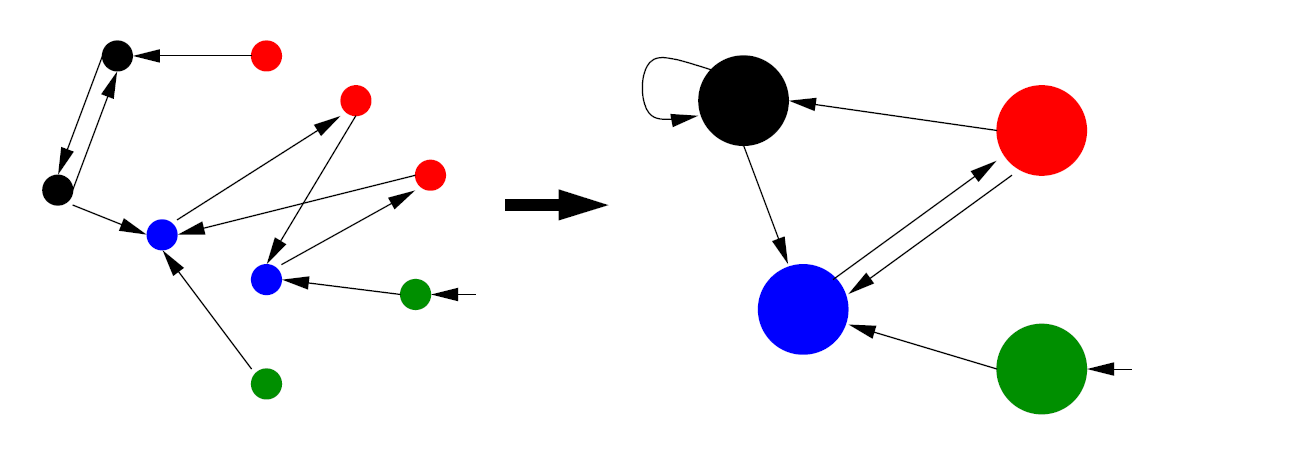
\includegraphics[width=\textwidth]{content/chapter_model_checking/software_model_checking/img/abstract.png}

\end{frame}

% ---------------------------------------------------------------------

\begin{frame}{Abstract Model Checking}
\begin{itemize}
  \itemsep1em
   
  \item Assume an abstract model $S_a$ of the concrete model $S_c$ such that
    $S_a \models \varphi \Rightarrow S_c \models \varphi$
  
  \item If a counterexample found in $S_a$, i.e. $S_a \models \neg \varphi$,
  then the abstract model has to be refined
  
  \item Refinement is repeated until the property is found to be true or a
  concrete a concrete counterexanple is found
  
  \item An abstract model $S_a$ is built using the \hl{Predicate abstraction}
  technique
  
  \item \hl{Counterexample-Guided Abstraction Refinement} (CEGAR)  
\end{itemize}
\end{frame}

% ---------------------------------------------------------------------

\begin{frame}{CEGAR}
\resizebox{1.05\textwidth}{!}{
  	\begin{tikzpicture}[>=stealth',shorten >=1pt,auto, node distance=3cm]
	 	\tikzstyle{rect} = [draw, rectangle, align=left,
	 	minimum width=2cm, minimum height=1cm]    
  			
  		\node[rect] (1) [] {Predicate \\ Abstraction};
  		\node[rect] (2) [right = of 1.east] {Model- \\ Checking};	
 		\node[rect] (3) [below of = 1] {Predicate \\ Refinement};
 		\node[rect] (4) [below of = 2] {Spurious ?};
 		
 		\node[node distance=1.8cm] (01) [left = of 1.west] {};
 		\node[node distance=1.8cm] (02) [right = of 2.east] {};
 		\node[node distance=1.8cm] (04) [right = of 4.east] {};
 		
 		\node[rectangle, draw, 
 		minimum width=7.6cm, minimum height=4.5cm, fit= (1) (2) (3) (4)] {};
 		
 		\path[->] 	(1)	edge node {Boolean program} (2)
 					(1)	edge[below] node {$\varphi$} (2)
 					
 					(2)	edge[left] node {Counter-example (CE)} (4)
 					(4)	edge[below] node {Spurious !} (3)
 					
 					(3)	edge[below] node {} (1)
 					
 					(01) edge node {Prog $P$} (1)
 					(01) edge[below] node {Spec $\varphi$} (1)
 					
 					(2) edge node {$\varphi$} (02)
 					
 					(4) edge node {$\neg \varphi$} (04)
 					(4) edge[below] node {CE} (04)					
 		; 					 				
	\end{tikzpicture}
  
}
\end{frame}

% ---------------------------------------------------------------------

\begin{frame}{CEGAR and Lazy Abstraction}
\resizebox{1.05\textwidth}{!}{
    \begin{tikzpicture}[>=stealth',shorten >=1pt,auto, node distance=3cm]
    \tikzstyle{rect} = [draw, rectangle, align=left,
    minimum width=2cm, minimum height=1cm]    
        
      \node[rect] (1) [] {\hl{Cartesian} \\ \hl{Abstraction}};
      \node[rect] (2) [right = of 1.east] {Explicit MC};  
    \node[rect] (3) [below of = 1] {\hl{Predicate} \\ \hl{Refinement}};
    \node[rect] (4) [below of = 2] {Spurious ?};
    
    \node[node distance=1.8cm] (01) [left = of 1.west] {};
    \node[node distance=1.8cm] (02) [right = of 2.east] {};
    \node[node distance=1.8cm] (04) [right = of 4.east] {};
    
    \node[rectangle, draw, 
    minimum width=7.6cm, minimum height=4.5cm, fit= (1) (2) (3) (4)] {};
    
    \path[->]   (1) edge node {$\hl{ART}$} (2)
          (2) edge[below] node {\hl{on-the-fly}} (1)
          
          (2) edge[left] node {Counter-example (CE)} (4)
          (4) edge[below] node {Spurious !} (3)
          
          (3) edge[below] node {} (1)
          
          (01) edge node {$\hl{CFA_\varphi}$} (1)        
          
          (2) edge node {$\varphi$} (02)
          
          (4) edge node {$\neg \varphi$} (04)
          (4) edge[below] node {CE} (04)          
    ;
          
          
  \end{tikzpicture}  
}
\end{frame}

% ---------------------------------------------------------------------

\begin{frame}{Control-Flow Automata (CFA)}
\begin{itemize}
  \itemsep1em 
  \item We consider simple imperative programs where all operations are either
  assignements or assume operations
  \item We represent a program by a \hl{control-flow automaton} $A =
  (L, G)$ where
    \begin{itemize}
      \itemsep 0.1cm 
      \item $L$ - is a set of program locations
      \item $G \subseteq L \times Ops \times L$ - is a set of control flow edges
  \end{itemize}
  \item A \hl{program} $P = (A, l_0, l_E)$ consist of a CFA $A = (L, G)$ and
  propgram locations $l_0, l_E \in L$ s.t.
    \begin{itemize}
      \itemsep 0.1cm
      \item $l_0$ - models an initial program location, and
      \item $l_E$ - models the error location
  \end{itemize}
  \item MC Problem: does the location $l_E$ is reachable from the location $l_0$
  in $P$
\end{itemize}
\end{frame}

% ---------------------------------------------------------------------

\begin{frame}[fragile]{Control-Flow Automata (CFA)}
\begin{columns}
  \begin{column}{0.6\textwidth}    
    \begin{overprint}
      \onslide<1-2>
        
\begin{figure}[htbp]
  \begin{center}
	\begin{tikzpicture}[>=stealth',shorten >=1pt,auto,node distance=1.2cm]
	 	
	 	 \onslide<1->{   	 	    
  			\node[loc] (1) []  	{$0$};		
  			\node[loc] (2) [below of = 1] 	{$1$};
 			  \node[loc] (3) [right of = 2, node distance=2cm]	{$2$};		
 			
 			  \node[loc] (4) [below of = 2]	{$3$};
 			  \node[loc] (5) [below of = 4]	{$4$};

        \path[trans]
          (1) edge [left] node {$i := 0$} (2)       
          (2) edge [left] node {$i > 5$} (4)

          (2) edge [above, bend left = 20] node {$i \leq 5$} (3)
          (3) edge [below, bend left = 20] node {$i := i + 1$} (2)          
          ;    		
 		} 		
 		
    \onslide<1>{
        \path[trans]
          (4) edge [left] node {$result := i$} (5)
        ;
    }

 		\onslide<2->{ 		
 			\node[loc] (6) [below of = 5]	{$5$};
 			\node[loc, fill=red!50] (7) [right of = 5]	{$\mathcal{E}$}; 		
 		}
 		 		
 		\onslide<2->{
 			\path[trans] 				
 				(5) edge [left] node {$result := i$} (6)
 			
 				(4) edge [left] node {$i = 6$} (5)
 				(4) edge [right] node {$i \neq 6$} (7)	
 			;		
 		}
 		
 		
	\end{tikzpicture}
  \end{center}
\end{figure}
    \end{overprint}
  \end{column}
  \begin{column}{0.4\textwidth}
    \begin{overprint}
    \onslide<1->
      \begin{example}   
        \begin{lstlisting}[escapechar=\%]
  i := 0
  while(i <= 5) {
    i := i + 1
  }
  result := i
        \end{lstlisting}
      \end{example}
    \onslide<2->{ 
      \hl{Assertion}: \\ $i = 6$ after the loop
    }
    \end{overprint} 
  \end{column}
\end{columns}
\end{frame}

% ---------------------------------------------------------------------

\begin{frame}{Control-Flow Automata (CFA)}
\begin{itemize}
  \itemsep1em 
  \item A \hl{concrete data state} of a program is a variable assignment $c:
  X \rightarrow D$ where $D$ is some non-empty domain
  
  \item We represent sets of concrete data states symbolically using first-order
  formulas \\
  \begin{itemize}
    \item an FO-formula $\varphi$ represents the set $S$ of all data states $c$
    that imply $\varphi$, i.e. $S = \{ c \ | \ c \models \varphi \}$
  \end{itemize}
  \item A \hl{concrete state} of a program is a pair $(l, c) \in L \times S$
  
  \item The \hl{concrete semantics} of an operation $op \in Ops$ is defined by
  the \hl{strongest postcondition} operator $SP_{op}$ as \\
    \begin{itemize}
      \itemsep 0.2cm 
      \item $SP_{x := e}(\varphi) = \exists x': \varphi_{[x \mapsto x' ]} \wedge
      (x = e_{[x \mapsto x']})$
      \item $SP_{p}(\varphi) = \varphi \wedge p$ where $p$ is a conditional, e.g. $i \leq 5$
    \end{itemize}
\end{itemize}

\end{frame}

% ---------------------------------------------------------------------

\begin{frame}{Cartesian Predicate Abstraction}
\begin{itemize}
  \itemsep1em 
  \item The \hl{predicate abstraction} domain is parameterized by a fixed
  finite set of first-order formulas $\pi$ with free variables from the
  program variables
  
  \item A \hl{cartesian predicate abstraction} $\varphi^\pi$ of a
  formula $\varphi$ is the strongest conjunction of predicates from
  $\pi$ that is entailed by $\varphi$:
    \begin{align*}
      \varphi^\pi := \bigwedge \{ p \in \pi \ | \ \varphi \Rightarrow p \}
    \end{align*}
  
  \item The abstract strongest postoperator $SP^\pi$ for the predicate
  abstraction $\pi$ is defined as:
    \begin{align*}
      SP_{op}^{\pi}(\varphi^\pi) =
      (SP_{op}(\varphi^\pi))^{\pi}
    \end{align*} 
\end{itemize}

\end{frame}

% ---------------------------------------------------------------------

\begin{frame}{Abstract Reachibility Tree (ART)}
\begin{itemize}
  \itemsep1em 
  
  \item An ART is a tree whose nodes are labeled with program locations and
  abstract states, i.e. $(l, \varphi^\pi)$
  
  \item A node $n = (l, \varphi)$ is \hl{covered} if there exists another
  node $n' = (l, \varphi')$ s.t. $\varphi' \models \varphi$
  
  \item An ART is \hl{complete} if every leaf node is covered
  
  \item Given a program $P = (A, l_0, l_E)$ and a set of predicates $\pi$,
  starting from the abstract state $(l_0, \{ \top \})$ we construct an
  \hl{abstract reachibility tree} (ART) using the abstract postoperator $SP^\pi$   
  
  \item If a complete ART is constructed and does not contain any error node
  $(l_E, \varphi)$, the program is considered correct
  
\end{itemize}
\end{frame}

% ---------------------------------------------------------------------

\begin{frame}{Abstract Reachibility Tree (ART)}
$\pi_0 = \{ i = 0\}$
\begin{columns}
  \begin{column}{0.5\textwidth}   
    
\begin{figure}[htbp]
  \begin{center}
	\begin{tikzpicture}[>=stealth',shorten >=1pt,auto,node distance=1.2cm]
		
		 	\node[loc] (1) []  	{$0$};		
  			\node[loc] (2) [below of = 1] 	{$1$};
 			\node[loc] (3) [right of = 2, node distance=2cm]	{$2$};		
 			
 			\node[loc] (4) [below of = 2]	{$3$};
 			\node[loc] (5) [below of = 4]	{$4$};
 			
 			\node[loc] (6) [below of = 5]	{$5$};
 			\node[loc, fill=red!50] (7) [right of = 5]	{$\mathcal{E}$};	 	
	 	 
	
 			\path[trans]  			
 				(1) edge [left] node {$i := 0$} (2)				
				(2) edge [left] node {$i > 5$} (4)									 						
 			;
 			

 			\path[trans]
 				(2) edge [above, bend left = 20] node {$i \leq 5$} (3)
 				(3) edge [below, bend left = 20] node {$i := i + 1$} (2)
 				
 				(5) edge [left] node {$result := i$} (6)
 			
 				(4) edge [left] node {$i = 6$} (5)
 				(4) edge [right] node {$i \neq 6$} (7)	
 			;				
 		
 		
	\end{tikzpicture}
  \end{center}
\end{figure}
  \end{column}  
  \begin{column}{0.5\textwidth}
    
\begin{figure}[htbp]
  \begin{center}
	\begin{tikzpicture}[>=stealth',shorten >=1pt,auto,node distance=1.2cm]
		
		 	\node[artloc={$\{ \}$}] (0) []  	{$0$};		
  			\node[artloc={$\{ i = 0 \}$}] (1) [below of = 0] 	{$1$};
 			\node[artloc={$\{ i = 0 \}$}] (2) [below of = 1]	{$2$};		
 			
 			\node[artloc={$\{ \}$}] (11) [below of = 2] 	{$1$};
 			
 			\node[artloc={$\{ \}$}] (3) [below of = 11]	{$3$};
 			
 			\node[artloc={$\{ \}$}, fill=red!50] (7) [below of = 3]	{$\mathcal{E}$};	 	
	 	 
	
 			\path[trans]  			
 				(0) edge [left] node {$i := 0$} (1)				
				(1) edge [left] node {$i \leq 5$} (2)
				(2) edge [left] node {$i := i + 1$} (11)				 						
 				(11) edge [left] node {$i > 5$} (3)
 				(3) edge [left] node {$i \neq 6$} (7)					
 			;				
 		
 		
	\end{tikzpicture}
  \end{center}
\end{figure}
  \end{column}
  
\end{columns}
\end{frame}

% ---------------------------------------------------------------------

\begin{frame}{Abstraction refinement}
\resizebox{1.05\textwidth}{!}{
  \begin{tikzpicture}[scale=0.75]

\tikzset{trans/.style={%
  ->,
  onslide=<2->{opacity=.1}
}}

\tikzset{atrans/.style={%
  ->,
  onslide=<3>{opacity=.1}
}}


\tikzset{cetrans/.style={%
  ->, 
  onslide=<3>{opacity=1}
}}


\tikzset{loc/.style={%
  state,
    minimum width=0.2cm,
    minimum height=0.2cm,
    onslide=<2->{opacity=.1}      
}}


\tikzset{celoc/.style={%
  state,
    minimum width=0.2cm,
    minimum height=0.2cm,
  onslide=<2>{opacity=.1}      
}}


\onslide<2->{
\fill[green!30]  plot[smooth cycle, tension=.7] coordinates 
  {(-14.5,2.5) (-13,1) (-11.5,1.5) (-13.5,3)};

\fill[pink]  plot[smooth cycle, tension=.7] coordinates 
  {(-4.5,6.5) (-1,5) (-1,6) (-4,7)};
 
\fill[blue!30]  plot[smooth cycle, tension=.7] coordinates {
  (-10.5,3) (-9.5,1) (-5,0.5) (-5,3) (-7,3.5)};
}


\onslide<2-3>{
\fill[yellow!50]  plot[smooth cycle,tension=.7] coordinates 
  {(-13,5) (-11.5,3.5) (-7.5,4.5) (-8.5,6.5) (-11.5,6)};

\fill[gray!50]  plot[smooth cycle, tension=.7] coordinates 
  {(-6.5,6) (-5.5,4) (-4,2.5) (-2.5,2) (-2,3.5) (-4,5) (-5,6.5)};
}

% Refined
\onslide<4->{
\fill[gray!50]  plot[smooth cycle, tension=.7] coordinates 
{(-5.5,5) (-5.5,4) (-4,2.5)(-2.5,2) (-2,3.5) (-3.5,4.5) (-4.5,5)};

\fill[yellow!50] plot[smooth cycle, tension=.7] coordinates 
{(-12.5,4) (-11.5,3.5) (-8.5,4) (-8.5,5) (-11.5,4.5)};

\fill[cyan!50]  plot[smooth cycle, tension=.7] coordinates 
{(-12,6) (-12,5) (-5,5.5) (-5,6.5) (-8.5,6.5)};
}



\node[loc, fill=green] (v13) at (-13.5,2.5) {};
\node[loc, fill=green] (v14) at (-12.5,1.5) {};
\node[loc, fill=red] (v9) at (-1.5,5.5) {};
\node[loc] (v6) at (-4.5,4) {};
\node[loc] (v11) at (-8.5,1.5) {};
\node[loc] (v12) at (-11.5,4) {};

\node[loc] (v3) at (-8.5,4.5) {};

\node[loc] (v10) at (-5.5,1.5) {};
\node[loc] (v7) at (-2.5,2.5) {};
\node[loc] (v8) at (-7,3) {};
\node[loc] (v15) at (-10,2.5) {};

% Counter-example
\node[celoc] (v1) at ((-11.5,5.5) {};
\node[celoc] (v2) at (-9,6) {};
\node[celoc] (v4) at (-5.5,6) {};
\node[celoc, fill=red] (v5) at (-3.5,6.5) {};

\draw[trans, cetrans]  (v1) edge (v2);


% Abstract transitions
% (yellow -> gray)
\draw[atrans, cetrans, onslide=<4->{opacity=.1}]  (v2) edge (v4); 
% (gray -> red)
\draw[atrans, cetrans]  (v4) edge (v5);
% (blue -> gray)
\draw[atrans]  (v10) edge (v7);
% (green -> yellow)
\draw[atrans]  (v13) edge (v12);
% (green -> blue)
\draw[atrans]  (v14) edge (v15);
% (yellow -> blue)
\draw[atrans]  (v3) edge (v8);


\draw[trans]  (v4) edge (v6);
\draw[trans]  (v6) edge (v7);
\draw[trans]  (v8) edge (v10);
\draw[trans]  (v11) edge (v10);
\draw[trans]  (v12) edge (v3);
\draw[trans]  (v15) edge (v8);
\draw[trans]  (v15) edge (v11);

%\draw[->]  (v12) edge (v1);

\end{tikzpicture}
}
\end{frame}

% ---------------------------------------------------------------------

\begin{frame}{Abstraction refinement}
\begin{itemize}
  \itemsep 1em 
  \item If during the construction of an ART we hit an error node, then we have
  to check whether the discovered path from the initial node $l_0$ to the error
  node $l_E$ exists in the concrete system
  
  \item The \hl{concrete semantics} for a program path 
  $\sigma = \langle (op_1, l_1), \ldots, (op_n, l_n) \rangle$, is defined as:
    \begin{align*}
      SP_\sigma(\varphi) = SP_{op_n}(\ldots SP_{op_1}(\varphi))
    \end{align*}
  
  \item A program path $\sigma$ is \hl{feasible} if $SP_\sigma(\top)$ is
  satisfiable, otherwise it is \hl{infeasible}
\end{itemize}
\end{frame}

% ---------------------------------------------------------------------

\begin{frame}{Abstraction refinement}
\begin{itemize}
  \itemsep 1em   
  \item If a discovered path is infeasible we have to refine the current
  abstraction, i.e. add new predicates to $\pi$
  
  \item In order to guarantee the termination of the algorithm the following 
  has to hold for the \underline{refined} set of predicates $\pi'$:
  \begin{align*}
      SP_{op_n}^{\pi'}(\ldots SP_{op_1}^{\pi'}(\top)) \models \bot
    \end{align*}
    
\end{itemize}
\end{frame}

% ---------------------------------------------------------------------

\begin{frame}{Abstraction refinement}
\begin{itemize}
  \itemsep 1em  
  \item We try to extract new predicates from the counterexample s.t.
    \begin{itemize}
      \itemsep 0.1cm
      \item the same counterxample will no be discovered in next interations
      \item predicates should be as precise as possible
      \item as few predicates as possible*
    \end{itemize}  
  \item There are two main techniques
    \begin{itemize}
      \itemsep 0.1cm
      \item Interpolants
      \item Weakest Preconditions / Strongest Postconditions
    \end{itemize}  
  \item Iterpolantion is the most widely used technique in all state of the art
  software model-checking tools (BLAST, CPAchecker)
    \begin{itemize}
      \itemsep 0.1cm
      \item mostly used for problems encoded over LRA theory
      \item lose of precision for the BV theory
      \item for the McCarthy's theory of arrays inapplicable princpially
    \end{itemize}        
\end{itemize}
\end{frame}

% ---------------------------------------------------------------------

\begin{frame}{Abstraction refinement}
\begin{itemize}
  \itemsep 0.3cm 
  \item Given a spurious counterexample $\sigma = \langle (op_1, l_1), \ldots,
  (op_n, l_n) \rangle$
  
  \item We define the refined set of predicates $\pi'$ as
  \begin{align*}
  \pi' = \pi \cup \bigcup_{i \in 1..n} \neg WP_{op_i}(\top) 
  \end{align*}  
  where
  \begin{align*}
  WP_{op_i}(\varphi) = WP(op_i, WP(op_{i + 1}, \ldots WP(op_n, \varphi))) 
  \end{align*}
  \item The weakest precondition operator is defined as:
      \begin{itemize}
      \itemsep 0.2cm 
      \item $WP_{x := e}(\varphi) = \varphi_{[x \mapsto e ]}$
      \item $WP_{p}(\varphi) = \varphi \wedge p$ where $p$ is a conditional, e.g. $i \leq 5$
    \end{itemize}    
\end{itemize}
\end{frame}

% ---------------------------------------------------------------------

\begin{frame}{Example 1}


\begin{figure}[htbp]
	\begin{tikzpicture}[>=stealth',shorten >=1pt,auto,node distance=2cm]
	 	
	 	\node (0) {ART$_0$: };
	 	
	 	\node[artloc={$\{ \}$}, node distance = 1cm] (1) 
	 		[right of = 0]	{$1$};
	 				
  		\node[artloc={$\{ \}$}] (2) 
  			[right of = 1] 	{$2$};	
 		
 		\node[artloc={$\{ \}$}] (4) 
 			[right of = 2]	{$4$};
 		
 		\node[artloc={$\{ \}$}] (6) 
 			[right of = 4]	{$\mathcal{E}$};
 				 
		\path[trans]  
 			
 			(1) edge node [below] {$i := 0$} 	(2)
			(2) edge node [below] {$i > 5$}		(4)	
			(4) edge node [below] {$i \neq 6$}	(6)		 									
 			;
 					
	\end{tikzpicture}
\end{figure}
\begin{itemize}
%   \item UNSAT-Core: \quad 
%   $i_1 = 0 \ \wedge \ i_2 = i_1 \ \wedge \ i_2 > 5$
  
  \item Compute WP for the following program: 
  \begin{gather*} 
  \onslide<5->{{\color{red} \{0 > 5 \wedge 0 \neq 6\}} } \\
  i := 0 \\
  \onslide<4->{ {\color{blue} \{ i > 5 \wedge i \neq 6 \} } }
  \\
  i > 5 \\
  \onslide<3->{ {\color{blue} \{ i \neq 6 \}} }
  \\
  i \neq 6 \\
  \onslide<2->{ {\color{blue} \{ \top \}} }
  \end{gather*}
  
  \item<5-> Extracted predicates: $\{ i = 6; \ i \leq 5 \vee i = 6 \}$
\end{itemize}
\end{frame}


% ---------------------------------------------------------------------

\begin{frame}{Example 2}
\begin{figure}
\resizebox{\textwidth}{!}{
  

\begin{tikzpicture}[>=stealth',shorten >=1pt,auto,node distance=1.7cm]
	 	
	 	\node (0) {ART$_1$: };
	 	
	 	\node[artloc={$\{ \}$}, node distance = 1cm] (1) 	
	 		[right of = 0]	{$1$};		
  		
  		\node[artloc={$\{i \leq 6\}$}] (2) 	
  			[right of = 1] 	{$2$};
  		
  		\node[artloc={$\{i \leq 6\}$}] (3) 	
  			[right of = 2] 	{$3$};
  		
  		\node[artloc={$\{\}$}] (22) 
  			[right of = 3, node distance = 2cm] 	{$2$};
 		
 		\node[artloc={$\{\}$}] (4) 
 			[right of = 22]	{$4$};
 		
 		\node[artloc={$\{\}$}] (6) 
 			[right of = 4]	{$\mathcal{E}$};
 				 
		\path[trans]  
 			
 			(1) edge node [below] {$i := 0$} 	(2)
 			(2) edge node [below] {$i \leq 5$}	(3)
			(3) edge node [below] {$i := i + 1$} (22)	
			(22) edge node [below] {$i > 5$}	(4)
			(4) edge node [below] {$i \neq 6$}	(6)	
 			;
 					
\end{tikzpicture}

}
\end{figure}

\begin{itemize}  
  \item Compute WP for the following program (short form):    
  \begin{gather*}
  \onslide<5->{{\color{red} \{ 0 + 1 > 5\}} } \\
  i := 0 \\
  \onslide<4->{{\color{blue} \{i + 1 > 5\}} } \\
  i := i + 1 \\
  \onslide<3->{ {\color{blue} \{ i > 5 \} } }
  \\
  i > 5 \\
  \onslide<2->{ {\color{blue} \{ \top \}} }
  \\
  \end{gather*} 
  \item<6-> Extracted predicates: $\{ i \leq 5; i \leq 4 \}$
  
\end{itemize}
\end{frame}


% CPAchecker
%!TEX root = ../../../main.tex

\newcommand\definergbcolor[2]{\definecolor{#1}{rgb}{#2}}
\newcommand\definecmykcolor[2]{\definecolor{#1}{cmyk}{#2}}

% Blue of the 'C' in the CPAchecker logo and the background of the SoSy-Lab logo
\definergbcolor{sosyblue}{0.3058823529411765 0.615686274509804 0.8392156862745098}
% Green of the checkmark in the CPAchecker logo
\definergbcolor{green}{0 0.63529414 0}
% Uni Passau colors, still needed for the 'P' and the 'A' in the CPAchecker logo
\definecmykcolor{uniorange}{0 0.5 1 0}
\definecmykcolor{unigrey}{0.08 0 0.06 0.47}

\newcommand\toolnamesize\smaller
\newcommand\tool[1]{{{\toolnamesize\scshape #1}\xspace}}
\newcommand\definetool[2]{\newcommand{#1}{\tool{#2}\xspace}}

%%%%%%%%%% TOOLS %%%%%%%%%%%%%%%%%%%
\definetool{\blast}       {Blast}
\definetool{\cpachecker}  {CPAchecker}
\definetool{\impact}      {Impact}

%%%%%%%%%% NOTATIONS %%%%%%%%%%
\newcommand{\kinduction}{\texorpdfstring{\textit{k}\protect\nobreakdash-induction}{k-induction}\xspace}

\newcommand{\cpacheckerurl}{https://cpachecker.sosy-lab.org}
%\newcommand{\cpacheckertitle}{\resizebox{!}{7mm}{% Created with inkscape
\documentclass{standalone}
\usepackage{../sosy-beamer}

\begin{document}
\begin{tikzpicture}[y=0.80pt, x=0.80pt, yscale=-1.000000, xscale=1.000000, inner sep=0pt, outer sep=0pt]
\begin{scope}[shift={(-221.97172,-411.62445)}]
  \begin{scope}[shift={(174.94262,35.80334)}]
    % Checkmark
    \path[fill=green] (343.2732,431.6103) .. controls (346.6213,431.6104) and
      (349.1539,434.3576) .. (350.8709,439.8519) .. controls (354.3049,450.1540) and
      (356.7516,455.3050) .. (358.2111,455.3049) .. controls (359.3271,455.3050) and
      (360.0397,454.0001) .. (361.2416,452.2830) .. controls (385.3654,413.6505) and
      (449.4021,378.7382) .. (451.7061,377.1931) .. controls (453.5563,375.7472) and
      (455.2449,375.7948) .. (457.7931,375.8348) .. controls (460.5402,375.8350) and
      (465.3567,378.5405) .. (466.3841,379.8938) .. controls (467.9207,382.1169) and
      (468.9861,381.3650) .. (470.1138,389.0872) .. controls (468.5352,393.5092) and
      (467.3858,393.7940) .. (466.3207,394.8515) .. controls (427.1214,422.0592) and
      (392.8516,441.3973) .. (364.5211,485.6959) .. controls (362.5465,488.7865) and
      (358.5115,490.3318) .. (352.4162,490.3318) .. controls (346.2350,490.3318) and
      (342.5863,490.0743) .. (341.4703,489.5591) .. controls (338.5514,488.2714) and
      (335.1174,481.7039) .. (331.1683,469.8565) .. controls (326.7041,456.7215) and
      (324.4719,448.4799) .. (324.4720,445.1317) .. controls (324.4719,441.5261) and
      (327.4767,438.0491) .. (333.4863,434.7009) .. controls (337.1778,432.6406) and
      (340.4401,431.6104) .. (343.2732,431.6103);
    % Letter 'C'
    \path[fill=sosyblue] (119.3807,446.3865) -- (147.2947,454.8240) .. controls
      (145.4196,462.6522) and (142.4665,469.1912) .. (138.4354,474.4412) .. controls
      (134.4040,479.6912) and (129.3884,483.6521) .. (123.3885,486.3240) .. controls
      (117.4353,488.9959) and (109.8415,490.3318) .. (100.6072,490.3318) .. controls
      (89.4041,490.3318) and (80.2400,488.7146) .. (73.1150,485.4803) .. controls
      (66.0369,482.1990) and (59.9197,476.4568) .. (54.7635,468.2537) .. controls
      (49.6072,460.0506) and (47.0291,449.5506) .. (47.0291,436.7537) .. controls
      (47.0291,419.6913) and (51.5525,406.5897) .. (60.5994,397.4490) .. controls
      (69.6931,388.2616) and (82.5369,383.6679) .. (99.1307,383.6678) .. controls
      (112.1150,383.6679) and (122.3103,386.2929) .. (129.7166,391.5428) .. controls
      (137.1696,396.7928) and (142.7009,404.8553) .. (146.3104,415.7303) --
      (118.1854,421.9881) .. controls (117.2009,418.8475) and (116.1697,416.5506) ..
      (115.0916,415.0974) .. controls (113.3103,412.6600) and (111.1306,410.7850) ..
      (108.5525,409.4724) .. controls (105.9744,408.1600) and (103.0915,407.5038) ..
      (99.9041,407.5037) .. controls (92.6853,407.5038) and (87.1541,410.4100) ..
      (83.3104,416.2224) .. controls (80.4041,420.5350) and (78.9509,427.3084) ..
      (78.9510,436.5428) .. controls (78.9509,447.9803) and (80.6853,455.8318) ..
      (84.1541,460.0974) .. controls (87.6228,464.3162) and (92.4978,466.4256) ..
      (98.7791,466.4256) .. controls (104.8728,466.4256) and (109.4665,464.7147) ..
      (112.5604,461.2928) .. controls (115.7009,457.8709) and (117.9743,452.9022) ..
      (119.3807,446.3865);
    % Letter 'P'
    \path[fill=uniorange] (152.5188,387.2537) -- (205.4641,387.2537) .. controls
      (216.9953,387.2538) and (225.6203,389.9960) .. (231.3391,395.4803) .. controls
      (237.1046,400.9647) and (239.9874,408.7694) .. (239.9875,418.8943) .. controls
      (239.9874,429.3006) and (236.8468,437.4334) .. (230.5657,443.2928) .. controls
      (224.3312,449.1522) and (214.7922,452.0819) .. (201.9485,452.0818) --
      (184.5110,452.0818) -- (184.5110,490.3318) -- (152.5188,490.3318) --
      (152.5188,387.2537)(184.5110,431.1990) -- (192.3157,431.1990) .. controls
      (198.4562,431.1991) and (202.7687,430.1444) .. (205.2532,428.0349) .. controls
      (207.7375,425.8788) and (208.9797,423.1366) .. (208.9797,419.8084) .. controls
      (208.9797,416.5741) and (207.9016,413.8319) .. (205.7454,411.5818) .. controls
      (203.5891,409.3319) and (199.5344,408.2069) .. (193.5813,408.2068) --
      (184.5110,408.2068) -- (184.5110,431.1990);
    % Letter 'A'
    \path[fill=unigrey] (294.4918,473.3162) -- (258.2105,473.3162) --
      (253.2183,490.3318) -- (220.6636,490.3318) -- (259.4058,387.2537) --
      (294.1402,387.2537) -- (332.8824,490.3318) -- (299.5543,490.3318) --
      (294.4918,473.3162)(287.8121,451.0271) -- (276.4214,413.9724) --
      (265.1011,451.0271) -- (287.8121,451.0271);
  \end{scope}
\end{scope}

\end{tikzpicture}
\end{document}

}\enspace \cpachecker}
\newcommand{\cpacheckertitle}{\cpachecker}

\tikzfading[name=arrowfading, top color=transparent!0, bottom color=transparent!95]
\tikzset{arrowfill/.style={top color=#1!30, bottom color=#1, general shadow={fill=black, shadow yshift=-0.4ex, path fading=arrowfading}}}
\tikzset{arrowstyle/.style n args={3}{single arrow, draw, arrowfill={#3}, minimum width=#1, minimum height=#2}}
\tikzset{%
  every node/.style={align=left, font=\small},
  tikzcpabar/.pic={
    % blue arrow
    \node[arrowstyle={0cm}{10cm}{sosyblue}, single arrow head extend=0.1cm, inner sep=1pt, rotate={#1}] at (0,0) (blueArrow) {};

    % left orange bar
    \node[arrowstyle={0.4cm}{0.6cm}{orange}, single arrow head extend=0cm, rotate={#1+90}] at ($(blueArrow.west) + (0.75,-0.4)$) {};

    % right orange bar
    \node[arrowstyle={0.4cm}{0.6cm}{orange}, single arrow head extend=0cm, rotate={#1+90}] at ($(blueArrow.east) + (-0.75,-0.4)$) {};

    % right lime-green arrow
    \node[arrowstyle={0cm}{2.5cm}{lime}, single arrow head extend=0.1cm, inner sep=3pt, rotate={#1}] at ($(blueArrow.center) + (1.25,-0.3)$) {};
    % left lime-green arrow
    \node[arrowstyle={0cm}{2.5cm}{lime}, single arrow head extend=0.1cm, inner sep=3pt, rotate={#1+180}] at ($(blueArrow.center) + (-1.25,-0.3)$) {};
    % green center bar
    \node[arrowstyle={0.4cm}{0.6cm}{green}, single arrow head extend=0cm, rotate={#1+90}] at ($(blueArrow.center) + (0,-0.4)$) {};
    }
  }

% Software Model Checking
%!TEX root = ../../../main.tex

\section{Software Model Checking with CPAchecker}

\begin{frame}{Software Model Checking with CPAchecker}
\begin{itemize}
\itemsep1em
\item \cpachecker is a versatile software verification tool created by SoSy-Lab
\item One of the world's most powerful and efficient verification tool
\item Web: \cpacheckerurl
\item Material of this section is based on the materials provided by developers of \cpachecker and is licensed under CC-BY-SA 4.0 
\end{itemize}

\end{frame}
 
% -----------------------

\begin{frame}{Software Verification}
  \small  
  \begin{minipage}{\textwidth}
    \documentclass[preview]{standalone}
\usepackage{../sosy-beamer}

\begin{document}
  \begin{tikzpicture}[
    every node/.style={
      align=left},
    arrowNode/.style={
      single arrow,
      draw,
      minimum height=0.7cm,
      single arrow head extend=0.1cm,
      inner sep=3pt,
      top color=sosyblue!30,
      bottom color=sosyblue}]

    \node (nodeDesc) {C Program};
    \node (nodeAlg) [draw, font=\ttfamily, font=\small, below = 0cm of nodeDesc] {
      int main() \{\\
      \quad int a = foo();\\
      \quad int b = bar(a);\\
      \\
      \quad assert(a == b);\\
      \}
    };

    \node (nodeArrLeft) [arrowNode, right = 0.35cm of nodeAlg] {};

    \node (nodeVerif) [align=center, draw, right = 0.35cm of nodeArrLeft] {Verification\\Tool};

    \node (nodeArrURight) [arrowNode, rotate=30, above right = -0.25cm and 0.5cm of nodeVerif] {};
    \node (nodeSafe) [align=left, right = 0.25cm of nodeArrURight] {\textcolor{green}{\large{TRUE}}\\\vspace{-0.4em}i.e., specification\\is satisfied};

    \node (nodeArrLRight) [arrowNode, rotate=-30, below right = -0.25cm and 0.5cm of nodeVerif] {};
    \node (nodeSafe) [align=left, below right = -0.15cm and 0.5cm of nodeArrLRight] {\textcolor{red}{FALSE}\\\vspace{-0.4em}i.e., bug found};

  \end{tikzpicture}
\end{document}

  \end{minipage}
  
  \bigskip
  \begin{minipage}{0.45\textwidth}
    General method:\\
    Create an overapproximation of the program states / \\
    compute program invariants
  \end{minipage}
    \hspace{0.2cm}
  \begin{minipage}{0.5\textwidth}
    \resizebox{\textwidth}{!}{
      \documentclass[preview]{standalone}
\usepackage{../sosy-beamer}

\begin{document}
  \begin{tikzpicture}[
  ellipseNode/.style={
    ellipse,
    draw,
    on grid,
    minimum width = 5cm,
    minimum height = 3.5cm,
    fill = sosyblue},
  cloudNode/.style={
    cloud,
    cloud ignores aspect,
    draw,
    on grid,
    align = center},
  innerCloudNode/.style={
    cloudNode,
    cloud puffs=9.89,
    minimum width = 4cm,
    minimum height = 1.5cm,
    top color = sosyblue!20,
    bottom color = sosyblue!60},
  outerCloudNode/.style={
    cloudNode,
    cloud puffs=6.32,
    minimum width = 2.25cm,
    minimum height = 1.0cm,
    fill = black}]

    \node (nodeEllipse) [ellipseNode, label={[shift={(0ex,-6ex)}]Overapproximation}] {};

    \node (nodeInnerCloud) [innerCloudNode, below = 0.5cm of nodeEllipse] {Reachable\\States};

    \node (nodeOuterCloud) [outerCloudNode, below right = 1cm and 3.5cm of nodeEllipse] {\textcolor{white}{Error}\\\textcolor{white}{States}};
  \end{tikzpicture}
\end{document}
    }
  \end{minipage}
\end{frame}

% ---------------------------------------------------------------------

% \begin{frame}{CPAchecker History}
%   \begin{itemize}
%     \item 2002: BLAST with lazy abstraction refinement
%     \item 2003: Multi-threading support
%     \item 2004: Test-case generation, interpolation, spec. lang.
%     \item 2005: Memory safety, predicated lattices
%     \item 2006: Lazy shape analysis
%     \item Maintenance and extensions became extremely difficult\\
%           because of design choices that were not easy to revert
%     \item 2007: Configurable program analysis,\\
%                 \cpachecker was started\\
%                 as complete reimplementation from scratch
%   \end{itemize}
% \end{frame}

% ---------------------------------------------------------------------

% \begin{frame}{CPAchecker History (2)}
%   \begin{itemize}
%     \item 2009: Large-block encoding
%     \item 2010: Adjustable-block encoding
%     \item 2012: Conditional model checking, PredAbs vs. Impact
%     \item 2013: Explicit-state MC, BDDs, precision reuse
%     \item ...
%   \end{itemize}
% \end{frame}

% ---------------------------------------------------------------------

\begin{frame}{Software Verification by Model Checking\\
  \vspace{-0.25cm}\small{[Clarke/Emerson, Sifakis 1981]}}
  \centering
  Iterative fixpoint (forward) post computation

  \medskip
  \begin{minipage}[b]{0.8\textwidth}
    \resizebox{\textwidth}{!}{
      \documentclass[preview]{standalone}
\usepackage{../sosy-beamer}

\begin{document}
  \begin{tikzpicture}
  \tikzset{custEllipse/.style={ellipse, draw}}

  % r_outer
  \onslide<4-4>{
    \node[custEllipse, fill=blue!20, text height =4cm, minimum width = 10cm,label={[anchor=south east,above=2mm]315:R}] (r-outer) {};
  }

  % r2
  \onslide<3-4>{
    \node[custEllipse, fill=blue!40, text height = 2.5cm, minimum width = 7cm, xshift=-0.75cm, yshift=0.4cm,label={[anchor=south,above=2mm]315:$R_2$}] at (r-outer.center) (r2) {};
  }

  % r1
  \onslide<2-4>{
    \node[custEllipse, fill=blue!60, text height = 1.5cm, minimum width = 4cm, xshift=-0.75cm, yshift=0.4cm, label={[anchor=south,above=2mm]315:$R_1$}] at (r2.center) (r1) {};
  }

  % r0
  \onslide<1-4>{
    \node[custEllipse, fill=blue!90, text height = 0.8cm, minimum width = 2.5cm, xshift=-0.5cm, yshift=0.27cm, label={[anchor=center,below=4mm]$R_0$}] at (r1.center) {};
  }

  % dots from r2 to r_outer
  \onslide<4-4>{
    \path ($(r2.south east) + (-0.5,0)$) -- ($(r-outer.south east) + (-0.75, 0)$) node [font=\huge, midway, sloped] {$\dots$};
  }
  \end{tikzpicture}
\end{document}
    }
  \end{minipage}
\end{frame}

% ---------------------------------------------------------------------

\begin{frame}<1>[label=algorithm]
  \frametitle{
    \only<1-2>{Software Model Checking}
    \only<3>{Configurable Program Analysis}}
  \begin{algorithmic}
    \State \textit{Reached}, \textit{Frontier} := $\{\text{\textit{e}}_\text{\textit{0}}\}$
    \While{\textit{Frontier} $\neq \emptyset$}
      \State remove \textit{e} from \textit{Frontier}
      \ForAll{\textit{e'} $\in$ \textbf{\underline{post}}(\textit{e})}
      \uncover<3->{
        \ForAll{\textit{e''} $\in$ \textit{Reached}}
          \State $\text{\textit{e''}}_{\text{\textit{new}}}$ := \textbf{\underline{merge}}(\textit{e'}, \textit{e''})
          \If{$\text{\textit{e''}}_{\text{\textit{new}}} \neq$ \textit{e''}}
            \State replace \textit{e''} in \textit{Reached}, \textit{Frontier} by   $\text{\textit{e''}}_{\text{\textit{new}}}$
          \EndIf
        \EndFor
      } %end uncover
        \If{$\neg$\textbf{\underline{stop}}(\textit{e'}, \textit{Reached})}
          \State add \textit{e'} to \textit{Reached}, \textit{Frontier}
        \EndIf
      \EndFor
    \EndWhile
  \State \Return \textit{Reached}
  \end{algorithmic}

\end{frame}

% ---------------------------------------------------------------------

\begin{frame}{Software Verification by Data-Flow Analysis}
  \centering
  Fixpoint computation on the CFG

  \begin{minipage}[b]{0.5\textwidth}
    \resizebox{\textwidth}{!}{
      \documentclass[preview]{standalone}
\usepackage{../sosy-beamer}

\begin{document}
  \begin{tikzpicture}
  \tikzset{orangebox/.style={rectangle, draw, fill=orange!60, minimum width = 2cm, minimum height = 1.5cm}}
  \tikzset{bluecircle/.style={circle, draw, fill=blue!60, minimum height = 1cm}}
  \tikzset{violetcircle/.style={circle, draw, fill=violet!80, minimum height = 1cm}}

  % draw orange boxes
  \foreach[count=\i] \posX/\posY in {2/6, 0/3, 4/3, 2/0} {
    \node[orangebox] (box\i) at (\posX,\posY) {};
  }

  \pgfmathtruncatemacro{\N}{9}

  % draw blue circles
  \foreach[count=\i] \n in {2,...,5}{
    \onslide<\n-\N>{
      \node[bluecircle] (circle) [on grid, below right = -0.5cm and -0.5cm of box\i.south east] {};
    }
  }

  % draw purple circles
  \foreach[count=\i] \n in {6,...,\N}{
    \onslide<\n-\N>{
      \node[violetcircle] (circle) [on grid, below right = -0.5cm and -0.5cm of box\i.south east] {};
    }
  }

  \foreach \from/\to in {box1/box2, box1/box3, box2/box4, box3/box4} {
    \draw[->, line width=0.3mm] (\from.south) to (\to.north);
  }

  \draw[->, line width=0.3mm] (box4.south) -- (2,-1) -- (-1.5,-1) -- (-1.5,7) -- (2,7) -- (box1.north);
\end{tikzpicture}
\end{document}
    }
  \end{minipage}
\end{frame}


\againframe<2>{algorithm}


\againframe<3>{algorithm}


\begin{frame}{Configurable Program Analysis}
  \begin{itemize}
    \item Better combination of abstractions\\
    \textbf{$\rightarrow$} Configurable Program Analysis  \hspace{0.1cm}\textcolor{sosyblue}{\tiny{[Beyer/Henzinger/Theoduloz CAV'07]}}
  \end{itemize}

  \medskip
  \begin{minipage}[b]{\textwidth}{
    \begin{tikzpicture}

      \pic [local bounding box=A1] at (0,1.5) {tikzcpabar={0}} ;
      \node [below = 0cm of A1] {CPA} ;

      \node [below left = 0cm and -3cm of A1] {Data-flow analysis} ;
      \node [below right = 0cm and -3cm of A1] {Model Checking} ;

      \node [above left = 0cm and -1.5cm of A1] {\textcolor{red}{Imprecise}\\\textcolor{green}{Scalable}} ;
      \node [above right = 0cm and -1.5cm of A1]  {\textcolor{green}{Precise}\\\textcolor{red}{Expensive}} ;

    \end{tikzpicture}
  }

  \vspace{1.5cm}
  Unified framework that enables intermediate algorithms
\end{minipage}
\end{frame}

% ---------------------------------------------------------------------

\begin{frame}{Dynamic Precision Adjustment}
Lazy abstraction refinement:\hspace{0.1cm}\textcolor{sosyblue}{\tiny{[Henzinger/Jhala/Majumdar/Sutre POPL'02]}}
\begin{itemize}
  \item Different predicates per location and per path
  \item Incremental analysis instead of restart from scratch after refinement
\end{itemize}
\end{frame}

% ---------------------------------------------------------------------

\begin{frame}{Dynamic Precision Adjustment}
  \begin{minipage}{0.55\textwidth}
    Better fine tuning of the precision of abstractions\\\vspace{-0.3em}
    $\rightarrow$ Adjustable Precision\\
    \textcolor{sosyblue}{\scriptsize{[Beyer/Henzinger/Theoduloz ASE'08]}}

    \bigskip
    Unified framework enables:
    \begin{itemize}
      \item switch on and off different analysis, and can
      \item adjust each analysis separately
    \end{itemize}

  \bigskip
  $\bullet$ Not only \textbf{refine}, also \textbf{abstract}!
  \end{minipage}
  \hspace{1cm}
  \begin{minipage}{0.3\textwidth}{
    \begin{tikzpicture}[scale=0.8, every node/.style={align=left, scale=0.8}]

      \pic [local bounding box=A2, rotate=90] {tikzcpabar={90}} ;
      \node [right of = A2] {CPA} ;

      \node [above right = -1cm and 0.5cm of A2] {\textcolor{red}{Imprecise}\\\textcolor{green}{Scalable}} ;
      \node [below right = -1cm and 0.5cm of A2]  {\textcolor{green}{Precise}\\\textcolor{red}{Expensive}} ;

    \end{tikzpicture}
    }
  \end{minipage}
\end{frame}

% ---------------------------------------------------------------------

\begin{frame}{Adjustable Block-Encoding}
  \begin{itemize}
    \item Handle loop-free blocks of statements at once
    \item Abstract only between blocks\\ (less abstractions, less refinements)\\
              \textcolor{sosyblue}{\scriptsize{[Beyer/Cimatti/Griggio/Keremoglu/Sebastiani FMCAD'09]}}\\
              \textcolor{sosyblue}{\scriptsize{[Beyer/Keremoglu/Wendler FMCAD'10]}}

  \end{itemize}
  %\hspace{9em}
  \bigskip
  \centering
  \begin{minipage}[b]{0.6\textwidth}  
    \resizebox{\textwidth}{!}{
      \begin{tikzpicture}

      \pic [local bounding box=A3, rotate=225] {tikzcpabar={225}} ;
      \node [below right = 0cm and 0cm of A3.center] {Block size} ;

      \node [above right = -1cm and 0cm of A3] {\textcolor{red}{SBE}} ;
      \node [below left = -0.5cm and -4cm of A3] {\textcolor{blue}{Whole Program}} ;

      \end{tikzpicture}
    }
  \end{minipage}
\end{frame}

% ---------------------------------------------------------------------

\begin{frame}<3->{\cpachecker}
              \textcolor{sosyblue}{\scriptsize{[Beyer/Keremoglu CAV'11]}}
%  \begin{tikzpicture}
  
  \bigskip
  \centering
  \begin{minipage}[b]{\textwidth}
    \resizebox{\textwidth}{!}{
      \begin{tikzpicture}
      \pic [local bounding box=A1] {tikzcpabar={0}} ;
      \node [below = 0cm of A1] {CPA} ;

      \pause
      \pic [local bounding box=A2, rotate=90, scale=0.8, every node/.style={scale=0.8}] at (1,0) {tikzcpabar={90}} ;

      \pause
      \pic [local bounding box=A3, rotate=225] at (2,0) {tikzcpabar={225}};
    \end{tikzpicture}
    }
  \end{minipage}
\end{frame}

% ---------------------------------------------------------------------

\begin{frame}{CPA -- Summary}
  \begin{itemize}
    \item Unification of several approaches\\
    $\rightarrow$ reduced to their essential properties
    \item Allow experimentation with new configurations\\ that we could never think of
    \item Flexible implementation \cpachecker
  \end{itemize}
\end{frame}

% ---------------------------------------------------------------------

\begin{frame}{\cpacheckertitle}
  \begin{itemize}
    \item Framework for Software Verification --- current status
    \begin{itemize}
      \item Written in Java
      \item Open Source: Apache 2.0 License
      \item \textasciitilde80 contributors so far from 15 universities/institutions
      \item 430.000 lines of code\\
      (275.000 without blank lines and comments)
      \item Started 2007
    \end{itemize}
  \end{itemize}
  \bigskip
  \centering\url{\cpacheckerurl}
\end{frame}

% ---------------------------------------------------------------------

\begin{frame}{\cpacheckertitle: Features}
  \begin{itemize}
    \item Input language C (experimental: Java)
    \item Web frontend available:\\
    \url{https://cpachecker.appspot.com}
    \item Counterexample output with graphs
    \item Benchmarking infrastructure available\\
    (with large cluster of machines)
    \item Cross-platform: Linux, Mac, Windows
  \end{itemize}
\end{frame}

% ---------------------------------------------------------------------

\begin{frame}{\cpacheckertitle: Achievements}
\begin{itemize}
  \item Among world's best software verifiers:\\
  \smaller\url{https://sv-comp.sosy-lab.org/2018/results/}\larger
  \item Continuous success in competition since 2012\\
    (52 medals: 16x gold, 18x silver, 18x bronze)
  \item Awarded Gödel medal\\ by Kurt Gödel Society
    \begin{textblock*}{3cm}(6cm,4.2cm)%
      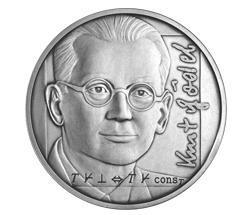
\includegraphics[width=3cm]{content/chapter_model_checking/cpachecker/images/goedel-medal}%
    \end{textblock*}%
    \bigskip
    \bigskip
    \bigskip
    \bigskip
  \item Used for Linux driver verification\\ with dozens of real bugs found and fixed in Linux
\end{itemize}
\end{frame}

% ---------------------------------------------------------------------

\begin{frame}{\cpacheckertitle: Concepts}
  \begin{itemize}
    \item Included Concepts:
    \begin{itemize}
      \item CEGAR
      \item Interpolation
      \item Adjustable-block encoding
      \item Conditional model checking
      \item Verification witnesses
    \end{itemize}
    \item Further available analyses:
    \begin{itemize}
      \item \impact algorithm
      \item Bounded model checking
      \item k-Induction
      \item Property-directed reachability
    \end{itemize}
  \end{itemize}
\end{frame}


% ---------------------------------------------------------------------

\begin{frame}{\cpacheckertitle: Concepts}
  \begin{itemize}
    \item Completely modular, and thus flexible and easily extensible
    \item Every abstract domain is implemented as a\\
    "Configurable Program Analysis" (CPA)
    \item E.g., predicate abstraction, explicit-value analysis, intervals, octagon, BDDs, memory graphs, and more
    \item Algorithms are central and implemented only once
    \item Separation of concerns
    \item Combined with Composite pattern
  \end{itemize}
\end{frame}

% ---------------------------------------------------------------------

\begin{frame}{\cpacheckertitle: Algorithms}
  \begin{itemize}
    \item CPAAlgorithm is the core algorithm\\ for reachability analysis / fixpoint iteration
    \item Other algorithms can be added if desired, e.g.,
    \begin{itemize}
      \item CEGAR
      \item Double-checking counterexamples
      \item Sequential combination of analyses
    \end{itemize}
  \end{itemize}
\end{frame}

% ---------------------------------------------------------------------

\begin{frame}[fragile]{\cpacheckertitle: Architecture}
  \resizebox{\textwidth}{!}{
    \documentclass[tikz]{standalone}
\usetikzlibrary{calc}
\usepackage{xspace}
\usepackage{xcolor}
\newcommand\definergbcolor[2]{\definecolor{#1}{rgb}{#2}}
\newcommand\definecmykcolor[2]{\definecolor{#1}{cmyk}{#2}}
\newcommand{\kinduction}{$k$-induction\xspace}
\newcommand{\kInduction}{$k$-Induction\xspace}
\begin{document}
\begin{tikzpicture}[line width=1pt]

\node[text width=1.5cm] (sourcecode) at ( 0cm,3.5cm) {\resizebox{1.5cm}{!}{\input{content/chapter_model_checking/cpachecker/images/document-sign}}};
\node[text width=1.5cm,align=center] (sourcecode-label) at (sourcecode) {Source Code};

\node[text width=1.5cm] (spec) at ( 0cm,0cm) {\resizebox{1.5cm}{!}{\input{content/chapter_model_checking/cpachecker/images/document-sign}}};
\node[text width=1.5cm,align=center] (spec-label) at (spec) {Spec};

\node[text width=1.5cm] (results) at (10cm,3.5cm) {\resizebox{1.5cm}{!}{\input{content/chapter_model_checking/cpachecker/images/document-sign}}};
\node[text width=1.5cm,align=center] (results-label) at (results) {Results};

\node[draw,text width=2cm,align=center,fill=sosyblue!20] (frontend)
 at (3cm, 3.5cm) {\mbox{Parser \&} \mbox{CFA Builder}};

\node[draw,text width=2cm,align=center,fill=green!60] (kindalgorithm)  at (6cm, 5.25cm) {\kinduction \mbox{Algorithm}};
\node[draw,text width=2cm,align=center,fill=green!60] (cegaralgorithm) at (6cm, 3.5cm) {CEGAR \mbox{Algorithm}};
\node[draw,text width=2cm,align=center,fill=green!60] (cpaalgorithm)   at (6cm, 1.75cm) {CPA \mbox{Algorithm}};

\node[draw,text width=1.5cm,align=center,fill=uniorange!60] (speccpa) at (3cm, 0cm) {Spec\\CPA};
\node[draw,text width=1.5cm,align=center,fill=uniorange!60] (loccpa) at (5cm, 0cm) {Location\\CPA};
\node[draw,text width=1.5cm,align=center,fill=uniorange!60] (callstackcpa) at (7cm, 0cm) {Callstack\\CPA};
\node[draw,text width=1.5cm, align=center,fill=uniorange!60] (predicatecpa) at (9cm, 0cm) {Predicate CPA};

\draw[->,double] (sourcecode) --(frontend);
\draw[->,double] (spec) --(speccpa);
\draw[->,double] (kindalgorithm) -|(results);
\draw[->,double] (cpaalgorithm) -|(results);

\draw[->] (frontend) |-(kindalgorithm);
\draw[->] (frontend) |-(cegaralgorithm);
\draw[->] (frontend) |-(cpaalgorithm);

\draw[->] (cpaalgorithm) --($(cpaalgorithm) - (0,0.75cm)$) -|(speccpa);
\draw[->] (cpaalgorithm) --($(cpaalgorithm) - (0,0.75cm)$) -|(loccpa);
\draw[->] (cpaalgorithm) --($(cpaalgorithm) - (0,0.75cm)$) -|(callstackcpa);
\draw[->] (cpaalgorithm) --($(cpaalgorithm) - (0,0.75cm)$) -|(predicatecpa);

\draw (kindalgorithm.south east) edge[bend left,->] (cpaalgorithm.north east);
\draw[->] (cegaralgorithm) --(cpaalgorithm);

\end{tikzpicture}
\end{document}

  }
\end{frame}

% ---------------------------------------------------------------------

% \begin{frame}{\resizebox{!}{7mm}{% Created with inkscape
\documentclass{standalone}
\usepackage{../sosy-beamer}

\begin{document}
\begin{tikzpicture}[y=0.80pt, x=0.80pt, yscale=-1.000000, xscale=1.000000, inner sep=0pt, outer sep=0pt]
\begin{scope}[shift={(-221.97172,-411.62445)}]
  \begin{scope}[shift={(174.94262,35.80334)}]
    % Checkmark
    \path[fill=green] (343.2732,431.6103) .. controls (346.6213,431.6104) and
      (349.1539,434.3576) .. (350.8709,439.8519) .. controls (354.3049,450.1540) and
      (356.7516,455.3050) .. (358.2111,455.3049) .. controls (359.3271,455.3050) and
      (360.0397,454.0001) .. (361.2416,452.2830) .. controls (385.3654,413.6505) and
      (449.4021,378.7382) .. (451.7061,377.1931) .. controls (453.5563,375.7472) and
      (455.2449,375.7948) .. (457.7931,375.8348) .. controls (460.5402,375.8350) and
      (465.3567,378.5405) .. (466.3841,379.8938) .. controls (467.9207,382.1169) and
      (468.9861,381.3650) .. (470.1138,389.0872) .. controls (468.5352,393.5092) and
      (467.3858,393.7940) .. (466.3207,394.8515) .. controls (427.1214,422.0592) and
      (392.8516,441.3973) .. (364.5211,485.6959) .. controls (362.5465,488.7865) and
      (358.5115,490.3318) .. (352.4162,490.3318) .. controls (346.2350,490.3318) and
      (342.5863,490.0743) .. (341.4703,489.5591) .. controls (338.5514,488.2714) and
      (335.1174,481.7039) .. (331.1683,469.8565) .. controls (326.7041,456.7215) and
      (324.4719,448.4799) .. (324.4720,445.1317) .. controls (324.4719,441.5261) and
      (327.4767,438.0491) .. (333.4863,434.7009) .. controls (337.1778,432.6406) and
      (340.4401,431.6104) .. (343.2732,431.6103);
    % Letter 'C'
    \path[fill=sosyblue] (119.3807,446.3865) -- (147.2947,454.8240) .. controls
      (145.4196,462.6522) and (142.4665,469.1912) .. (138.4354,474.4412) .. controls
      (134.4040,479.6912) and (129.3884,483.6521) .. (123.3885,486.3240) .. controls
      (117.4353,488.9959) and (109.8415,490.3318) .. (100.6072,490.3318) .. controls
      (89.4041,490.3318) and (80.2400,488.7146) .. (73.1150,485.4803) .. controls
      (66.0369,482.1990) and (59.9197,476.4568) .. (54.7635,468.2537) .. controls
      (49.6072,460.0506) and (47.0291,449.5506) .. (47.0291,436.7537) .. controls
      (47.0291,419.6913) and (51.5525,406.5897) .. (60.5994,397.4490) .. controls
      (69.6931,388.2616) and (82.5369,383.6679) .. (99.1307,383.6678) .. controls
      (112.1150,383.6679) and (122.3103,386.2929) .. (129.7166,391.5428) .. controls
      (137.1696,396.7928) and (142.7009,404.8553) .. (146.3104,415.7303) --
      (118.1854,421.9881) .. controls (117.2009,418.8475) and (116.1697,416.5506) ..
      (115.0916,415.0974) .. controls (113.3103,412.6600) and (111.1306,410.7850) ..
      (108.5525,409.4724) .. controls (105.9744,408.1600) and (103.0915,407.5038) ..
      (99.9041,407.5037) .. controls (92.6853,407.5038) and (87.1541,410.4100) ..
      (83.3104,416.2224) .. controls (80.4041,420.5350) and (78.9509,427.3084) ..
      (78.9510,436.5428) .. controls (78.9509,447.9803) and (80.6853,455.8318) ..
      (84.1541,460.0974) .. controls (87.6228,464.3162) and (92.4978,466.4256) ..
      (98.7791,466.4256) .. controls (104.8728,466.4256) and (109.4665,464.7147) ..
      (112.5604,461.2928) .. controls (115.7009,457.8709) and (117.9743,452.9022) ..
      (119.3807,446.3865);
    % Letter 'P'
    \path[fill=uniorange] (152.5188,387.2537) -- (205.4641,387.2537) .. controls
      (216.9953,387.2538) and (225.6203,389.9960) .. (231.3391,395.4803) .. controls
      (237.1046,400.9647) and (239.9874,408.7694) .. (239.9875,418.8943) .. controls
      (239.9874,429.3006) and (236.8468,437.4334) .. (230.5657,443.2928) .. controls
      (224.3312,449.1522) and (214.7922,452.0819) .. (201.9485,452.0818) --
      (184.5110,452.0818) -- (184.5110,490.3318) -- (152.5188,490.3318) --
      (152.5188,387.2537)(184.5110,431.1990) -- (192.3157,431.1990) .. controls
      (198.4562,431.1991) and (202.7687,430.1444) .. (205.2532,428.0349) .. controls
      (207.7375,425.8788) and (208.9797,423.1366) .. (208.9797,419.8084) .. controls
      (208.9797,416.5741) and (207.9016,413.8319) .. (205.7454,411.5818) .. controls
      (203.5891,409.3319) and (199.5344,408.2069) .. (193.5813,408.2068) --
      (184.5110,408.2068) -- (184.5110,431.1990);
    % Letter 'A'
    \path[fill=unigrey] (294.4918,473.3162) -- (258.2105,473.3162) --
      (253.2183,490.3318) -- (220.6636,490.3318) -- (259.4058,387.2537) --
      (294.1402,387.2537) -- (332.8824,490.3318) -- (299.5543,490.3318) --
      (294.4918,473.3162)(287.8121,451.0271) -- (276.4214,413.9724) --
      (265.1011,451.0271) -- (287.8121,451.0271);
  \end{scope}
\end{scope}

\end{tikzpicture}
\end{document}

}\enspace Try \cpachecker}
\begin{frame}{\cpacheckertitle: Try \cpachecker}
  \begin{itemize}
    \item Online at Google AppEngine:\\
    \url{https://cpachecker.appspot.com/}
    \item Download for Linux/Windows:\\
    \url{\cpacheckerurl}
    \begin{itemize}
      \item Run \texttt{scripts/cpa.sh} | \texttt{scripts$\backslash$cpa.bat}
      \item \texttt{-predicateAnalysis <FILE>}
      \item Windows/Mac need to disable bitprecise analysis:\\
        \texttt{-predicateAnalysis-linear\\ -setprop solver.solver=smtinterpol\\ -setprop analysis.checkCounterexamples=false}
    \end{itemize}
    \item Look at \texttt{output/CPALog.txt} for problems
    \item Open \texttt{.dot} files with dotty / xdot (\url{www.graphviz.org/})
    \item Open graphical report in browser: \texttt{output/*.html}
  \end{itemize}
\end{frame}

% ---------------------------------------------------------------------

\begin{frame}{\cpacheckertitle: Specification}
  \begin{itemize}
    \item Model Checkers check only what you specified
    \item \cpachecker's default:
    \begin{itemize}
      \item Label \texttt{ERROR}
      \item Calling function \_\texttt{assert\_fail()}
      \item \texttt{assert(pred)} needs to be pre-processed
    \end{itemize}
    \item SV-COMP:
    \begin{itemize}
      \item Calling function \_\texttt{VERIFIER\_error()}
      \item \texttt{-spec sv-comp-reachability}
    \end{itemize}
  \end{itemize}
\end{frame}

% ---------------------------------------------------------------------

\begin{frame}{\cpacheckertitle for Developers}
  Want to implement your own analysis?
  \begin{itemize}
    \item Easy, just write a CPA in Java
    \item Implementations for 10 interfaces needed
    \item But for 8, we have default implementations\\
      \textbf{$\rightarrow$} Minimal configuration: \\
      \qquad abstract state and\\
      \qquad abstract post operator
  \end{itemize}
\end{frame}

% ---------------------------------------------------------------------

\begin{frame}{\cpacheckertitle for Developers}
  The CPA framework is flexible:
  \begin{itemize}
    \item Many components are provided as CPAs:
      \begin{itemize}
        \item Location / program counter tracking
        \item Callstack tracking
        \item Specification input (as automata)
        \item Pointer-aliasing information
      \end{itemize}
    \item CPAs can be combined,\\
      so your analysis doesn't need to care about these things
  \end{itemize}
\end{frame}


% Conclusion
%!TEX root = ../../main.tex

\section{Conclusion}

\begin{frame}{Conclusion}
\begin{itemize}
\itemsep1em
\item Model Checking is an \hl{automatic} approach to \hl{verify} whether a given system satisfies a given specification
\item Proof of \hl{correctness} or \hl{counterexample} 
\item System properties: \hl{liveness, safety, invariants}
\item Symbolic Model Checking: make possible to handle infinite state systems and work around the state explosion problem
\item Over-/Under-approximation to abstract away superfluous information
\item Software Model Checking: no algorithm for all cases $\rightarrow$ combine different approaches    
\end{itemize}

\end{frame}

\mode<article>
\exercises

\mode
<all>